% Options for packages loaded elsewhere
\PassOptionsToPackage{unicode}{hyperref}
\PassOptionsToPackage{hyphens}{url}
\PassOptionsToPackage{dvipsnames,svgnames,x11names}{xcolor}
%
\documentclass[
]{agujournal2019}

\usepackage{amsmath,amssymb}
\usepackage{iftex}
\ifPDFTeX
  \usepackage[T1]{fontenc}
  \usepackage[utf8]{inputenc}
  \usepackage{textcomp} % provide euro and other symbols
\else % if luatex or xetex
  \usepackage{unicode-math}
  \defaultfontfeatures{Scale=MatchLowercase}
  \defaultfontfeatures[\rmfamily]{Ligatures=TeX,Scale=1}
\fi
\usepackage{lmodern}
\ifPDFTeX\else  
    % xetex/luatex font selection
\fi
% Use upquote if available, for straight quotes in verbatim environments
\IfFileExists{upquote.sty}{\usepackage{upquote}}{}
\IfFileExists{microtype.sty}{% use microtype if available
  \usepackage[]{microtype}
  \UseMicrotypeSet[protrusion]{basicmath} % disable protrusion for tt fonts
}{}
\makeatletter
\@ifundefined{KOMAClassName}{% if non-KOMA class
  \IfFileExists{parskip.sty}{%
    \usepackage{parskip}
  }{% else
    \setlength{\parindent}{0pt}
    \setlength{\parskip}{6pt plus 2pt minus 1pt}}
}{% if KOMA class
  \KOMAoptions{parskip=half}}
\makeatother
\usepackage{xcolor}
\setlength{\emergencystretch}{3em} % prevent overfull lines
\setcounter{secnumdepth}{5}
% Make \paragraph and \subparagraph free-standing
\makeatletter
\ifx\paragraph\undefined\else
  \let\oldparagraph\paragraph
  \renewcommand{\paragraph}{
    \@ifstar
      \xxxParagraphStar
      \xxxParagraphNoStar
  }
  \newcommand{\xxxParagraphStar}[1]{\oldparagraph*{#1}\mbox{}}
  \newcommand{\xxxParagraphNoStar}[1]{\oldparagraph{#1}\mbox{}}
\fi
\ifx\subparagraph\undefined\else
  \let\oldsubparagraph\subparagraph
  \renewcommand{\subparagraph}{
    \@ifstar
      \xxxSubParagraphStar
      \xxxSubParagraphNoStar
  }
  \newcommand{\xxxSubParagraphStar}[1]{\oldsubparagraph*{#1}\mbox{}}
  \newcommand{\xxxSubParagraphNoStar}[1]{\oldsubparagraph{#1}\mbox{}}
\fi
\makeatother


\providecommand{\tightlist}{%
  \setlength{\itemsep}{0pt}\setlength{\parskip}{0pt}}\usepackage{longtable,booktabs,array}
\usepackage{calc} % for calculating minipage widths
% Correct order of tables after \paragraph or \subparagraph
\usepackage{etoolbox}
\makeatletter
\patchcmd\longtable{\par}{\if@noskipsec\mbox{}\fi\par}{}{}
\makeatother
% Allow footnotes in longtable head/foot
\IfFileExists{footnotehyper.sty}{\usepackage{footnotehyper}}{\usepackage{footnote}}
\makesavenoteenv{longtable}
\usepackage{graphicx}
\makeatletter
\newsavebox\pandoc@box
\newcommand*\pandocbounded[1]{% scales image to fit in text height/width
  \sbox\pandoc@box{#1}%
  \Gscale@div\@tempa{\textheight}{\dimexpr\ht\pandoc@box+\dp\pandoc@box\relax}%
  \Gscale@div\@tempb{\linewidth}{\wd\pandoc@box}%
  \ifdim\@tempb\p@<\@tempa\p@\let\@tempa\@tempb\fi% select the smaller of both
  \ifdim\@tempa\p@<\p@\scalebox{\@tempa}{\usebox\pandoc@box}%
  \else\usebox{\pandoc@box}%
  \fi%
}
% Set default figure placement to htbp
\def\fps@figure{htbp}
\makeatother
% definitions for citeproc citations
\NewDocumentCommand\citeproctext{}{}
\NewDocumentCommand\citeproc{mm}{%
  \begingroup\def\citeproctext{#2}\cite{#1}\endgroup}
\makeatletter
 % allow citations to break across lines
 \let\@cite@ofmt\@firstofone
 % avoid brackets around text for \cite:
 \def\@biblabel#1{}
 \def\@cite#1#2{{#1\if@tempswa , #2\fi}}
\makeatother
\newlength{\cslhangindent}
\setlength{\cslhangindent}{1.5em}
\newlength{\csllabelwidth}
\setlength{\csllabelwidth}{3em}
\newenvironment{CSLReferences}[2] % #1 hanging-indent, #2 entry-spacing
 {\begin{list}{}{%
  \setlength{\itemindent}{0pt}
  \setlength{\leftmargin}{0pt}
  \setlength{\parsep}{0pt}
  % turn on hanging indent if param 1 is 1
  \ifodd #1
   \setlength{\leftmargin}{\cslhangindent}
   \setlength{\itemindent}{-1\cslhangindent}
  \fi
  % set entry spacing
  \setlength{\itemsep}{#2\baselineskip}}}
 {\end{list}}
\usepackage{calc}
\newcommand{\CSLBlock}[1]{\hfill\break\parbox[t]{\linewidth}{\strut\ignorespaces#1\strut}}
\newcommand{\CSLLeftMargin}[1]{\parbox[t]{\csllabelwidth}{\strut#1\strut}}
\newcommand{\CSLRightInline}[1]{\parbox[t]{\linewidth - \csllabelwidth}{\strut#1\strut}}
\newcommand{\CSLIndent}[1]{\hspace{\cslhangindent}#1}

\usepackage{booktabs}
\usepackage{caption}
\usepackage{longtable}
\usepackage{colortbl}
\usepackage{array}
\usepackage{url} %this package should fix any errors with URLs in refs.
\usepackage{lineno}
\usepackage[inline]{trackchanges} %for better track changes. finalnew option will compile document with changes incorporated.
\usepackage{soul}
\linenumbers
\makeatletter
\@ifpackageloaded{tcolorbox}{}{\usepackage[skins,breakable]{tcolorbox}}
\@ifpackageloaded{fontawesome5}{}{\usepackage{fontawesome5}}
\definecolor{quarto-callout-color}{HTML}{909090}
\definecolor{quarto-callout-note-color}{HTML}{0758E5}
\definecolor{quarto-callout-important-color}{HTML}{CC1914}
\definecolor{quarto-callout-warning-color}{HTML}{EB9113}
\definecolor{quarto-callout-tip-color}{HTML}{00A047}
\definecolor{quarto-callout-caution-color}{HTML}{FC5300}
\definecolor{quarto-callout-color-frame}{HTML}{acacac}
\definecolor{quarto-callout-note-color-frame}{HTML}{4582ec}
\definecolor{quarto-callout-important-color-frame}{HTML}{d9534f}
\definecolor{quarto-callout-warning-color-frame}{HTML}{f0ad4e}
\definecolor{quarto-callout-tip-color-frame}{HTML}{02b875}
\definecolor{quarto-callout-caution-color-frame}{HTML}{fd7e14}
\makeatother
\makeatletter
\@ifpackageloaded{caption}{}{\usepackage{caption}}
\AtBeginDocument{%
\ifdefined\contentsname
  \renewcommand*\contentsname{Table of contents}
\else
  \newcommand\contentsname{Table of contents}
\fi
\ifdefined\listfigurename
  \renewcommand*\listfigurename{List of Figures}
\else
  \newcommand\listfigurename{List of Figures}
\fi
\ifdefined\listtablename
  \renewcommand*\listtablename{List of Tables}
\else
  \newcommand\listtablename{List of Tables}
\fi
\ifdefined\figurename
  \renewcommand*\figurename{Figure}
\else
  \newcommand\figurename{Figure}
\fi
\ifdefined\tablename
  \renewcommand*\tablename{Table}
\else
  \newcommand\tablename{Table}
\fi
}
\@ifpackageloaded{float}{}{\usepackage{float}}
\floatstyle{ruled}
\@ifundefined{c@chapter}{\newfloat{codelisting}{h}{lop}}{\newfloat{codelisting}{h}{lop}[chapter]}
\floatname{codelisting}{Listing}
\newcommand*\listoflistings{\listof{codelisting}{List of Listings}}
\makeatother
\makeatletter
\makeatother
\makeatletter
\@ifpackageloaded{caption}{}{\usepackage{caption}}
\@ifpackageloaded{subcaption}{}{\usepackage{subcaption}}
\makeatother

\usepackage{bookmark}

\IfFileExists{xurl.sty}{\usepackage{xurl}}{} % add URL line breaks if available
\urlstyle{same} % disable monospaced font for URLs
\hypersetup{
  pdftitle={Distinct functional responses of producers and their consumers to climate shape trophic asymmetry in mutualistic networks},
  pdfauthor={Gabriel Munoz; Paul Savary; W. Daniel Kissling; JP Lessard},
  pdfkeywords={Climate change, Frugivory, Interaction diversity, Network
specialization, Seed dispersal},
  colorlinks=true,
  linkcolor={blue},
  filecolor={Maroon},
  citecolor={Blue},
  urlcolor={Blue},
  pdfcreator={LaTeX via pandoc}}


\journalname{Community Ecology}

\draftfalse

\begin{document}
\title{Distinct functional responses of producers and their consumers to
climate shape trophic asymmetry in mutualistic networks}

\authors{Gabriel Munoz\affil{1}, Paul Savary\affil{1}, W. Daniel
Kissling\affil{2}, JP Lessard\affil{1}}
\affiliation{1}{Concordia University, }\affiliation{2}{University of
Amsterdam, }
\correspondingauthor{Gabriel Munoz}{gabrielmunoz1891@gmail.com}


\begin{abstract}
Functional traits are often used to infer the ecological processes that
determine the composition of species assemblages. Whereas most
trait-based approaches to infer community assembly processes focus on a
single trophic level, traits also mediate interactions between trophic
levels. Owing to the matching of traits facilitating interactions
between producer and consumer assemblages, the functional trait
diversity of different trophic levels is expected to covary in space.
However, the differential response of consumers and producers to
environmental gradients can cause a decoupling of functional diversity
between trophic levels, which we coin functional trophic asymmetry.
Here, we develop a metric to quantify functional trophic asymmetry (FTA)
and use it to infer the processes underpinning multitrophic community
assembly and explore the role of these processes in shaping the topology
of ecological networks.

We used digitally available data on the functional traits, pairwise
mutualistic interactions, and geographic distributions of consumers
(mammalian frugivores) and their producers (palms) to quantify FTA for
species assemblages occurring in the Neotropics. To cover major data
gaps between species-level trait and interaction data at finer spatial
grain, we trained machine learning models to downscale the continental
meta-network to grid cell-level networks. For each grid-cell, we also
estimated FTA for all combinations of interaction guilds. These guilds
were defined as distinct subsets of producer and consumer assemblages
playing similar roles within mutualistic networks and sharing partners
in the other trophic level. We then used generalized additive models to
relate geographic variation in FTA to variation in climatic variables
and assessed whether the strength of these relationship varied among
pairwise interaction guilds. Finally, we then examined the relationship
between FTA and network specialization across 1,072 grid cells in the
Neotropics.

Our approach to model mutualistic network assembly identified 7
consumers x producer interaction guilds. Assemblage-wide FTA was
negatively related to annual mean temperatures across the neotropics.
When considering individual interaction guilds, precipitation
seasonality was positively related to FTA. This relationship between FTA
and precipitation seasonality was stronger for consumer and producer
guild combinations with high predicted interaction strength. Finally,
network specialization was positively related to FTA, regardless of the
interaction guild combination.

Mutualistic networks in warm regions with seasonal rainfall, where the
environment imposes a disproportionately strong selective pressure on
palms relative to mammal frugivores, exhibit higher levels of functional
trophic asymmetry. This relationship is particularly strong when
considering guilds predicted to strongly interact in nature. Assemblages
exhibiting high FTA also tend to have high levels of network
specialization, suggesting that differences in the strength of
environmental selection among trophic levels favor the persistence of
specialist species in these mutualistic interaction networks. We
therefore conclude that future increases in temperature and the
magnitude of precipitation seasonality caused by global climate change
could lead to more specialized mutualistic networks which are more prone
to collapse when facing further threats and local extinctions.
\end{abstract}





\subsection{Introduction}\label{introduction}

Ecologists often examine patterns of functional trait diversity to
investigate community assembly processes (Ackerly, 2003; Kraft et al.,
2015). To date, however, trait-based approaches in ecology often focus
on a single trophic level, whereas approaches that consider multiple
trophic levels remain rare (Lavorel, 2013; Seibold et al., 2018). An
approach that considers processes operating within and between trophic
levels is necessary to better understand the assembly of multitrophic
communities (Allesina et al., 2008; Marjakangas et al., 2022; Saravia et
al., 2022). Moreover, considering trophic interactions while studying
community assembly could shed new light on processes underpinning
ecological networks (Allesina et al., 2008). Classical approaches to
study community assembly rely on the concept of environmental filtering,
sorting or selection, where density independent conditions constrain the
functional richness of species assemblages (HilleRisLambers et al.,
2012; Kraft et al., 2015; Laliberté \& Legendre, 2010; Villéger et al.,
2008). Functional richness refers to the variability and relative
frequency of different functional traits observed in a community. It is
often used to estimate the strength of selection imposed by the
environment (Kraft et al., 2008, 2015; Kraft \& Ackerly, 2010). High
functional richness can indicate weak environmental selection whereas
low functional richness can indicate strong selection (Halpern \&
Floeter, 2008; Kraft et al., 2008; Paine et al., 2011). In a
multitrophic context, the effects of environmental selection can cascade
across trophic levels such that selection on consumer traits can shape
the functional richness of their resources, modulated by their degree of
reciprocal dependency or co-evolution (Lavorel, 2013). Moreover, the
same environmental gradient could exert selective pressures of different
strength on communities at distinct trophic levels (Marjakangas et al.,
2022). Differences in the strength of selective pressure among trophic
levels could then possibly constrain the structure or topologies of
trophic networks (Blüthgen et al., 2007; Dehling et al., 2021;
Schleuning et al., 2012)

Inferring the relative strength of environmental selection between
trophic levels requires using high-dimensional approaches that can deal
with sparse observations for many species (Rohr et al., 2010; Strydom et
al., 2022). We introduce the concept of functional trophic asymmetry
(FTA), which allows inferring the relative influence of environmental
selection and trait matching on the composition of multitrophic
assemblages (Figure~\ref{fig-01}). FTA is the difference in the richness
of interaction-relevant traits between trophic levels in a multitrophic
network. FTA can occur because traits mediating species interactions
(i.e., interaction niches) across trophic levels can also mediate the
responses of species to their abiotic environment (i.e., environmental
niches) (Dehling et al., 2021; McCain \& King, 2014; Moretti \& Legg,
2009). As an example, plant seed size determines the outcome of
animal-mediated seed dispersal (Donoso et al., 2017, 2020) as well as
physiological limits, such as tolerances of plant seedlings to
desiccation (Hoekstra et al., 2001). High FTA could indicate differences
in the strength of environmental selection over the interaction niches
of distinct trophic levels within a multitrophic species assemblage.
Alternatively, low FTA could indicate that the strength of the
environment selection shaping interaction niches is similar between
trophic levels, e.g., equally weak or equally strong (Marjakangas et
al., 2022). When interactions between producers and consumers are
mutualistic, low FTA could also emerge under strong trait matching and
therefore indicate the influence of trait co-evolution during
multitrophic community assembly (Albrecht et al., 2018; Dehling et al.,
2021). By studying spatial variation in FTA along environmental
gradients, we could possibly identify the conditions promoting
environmentally versus cross-trophic interaction- driven community
assembly (Bello et al., 2023).

\begin{figure}

\centering{

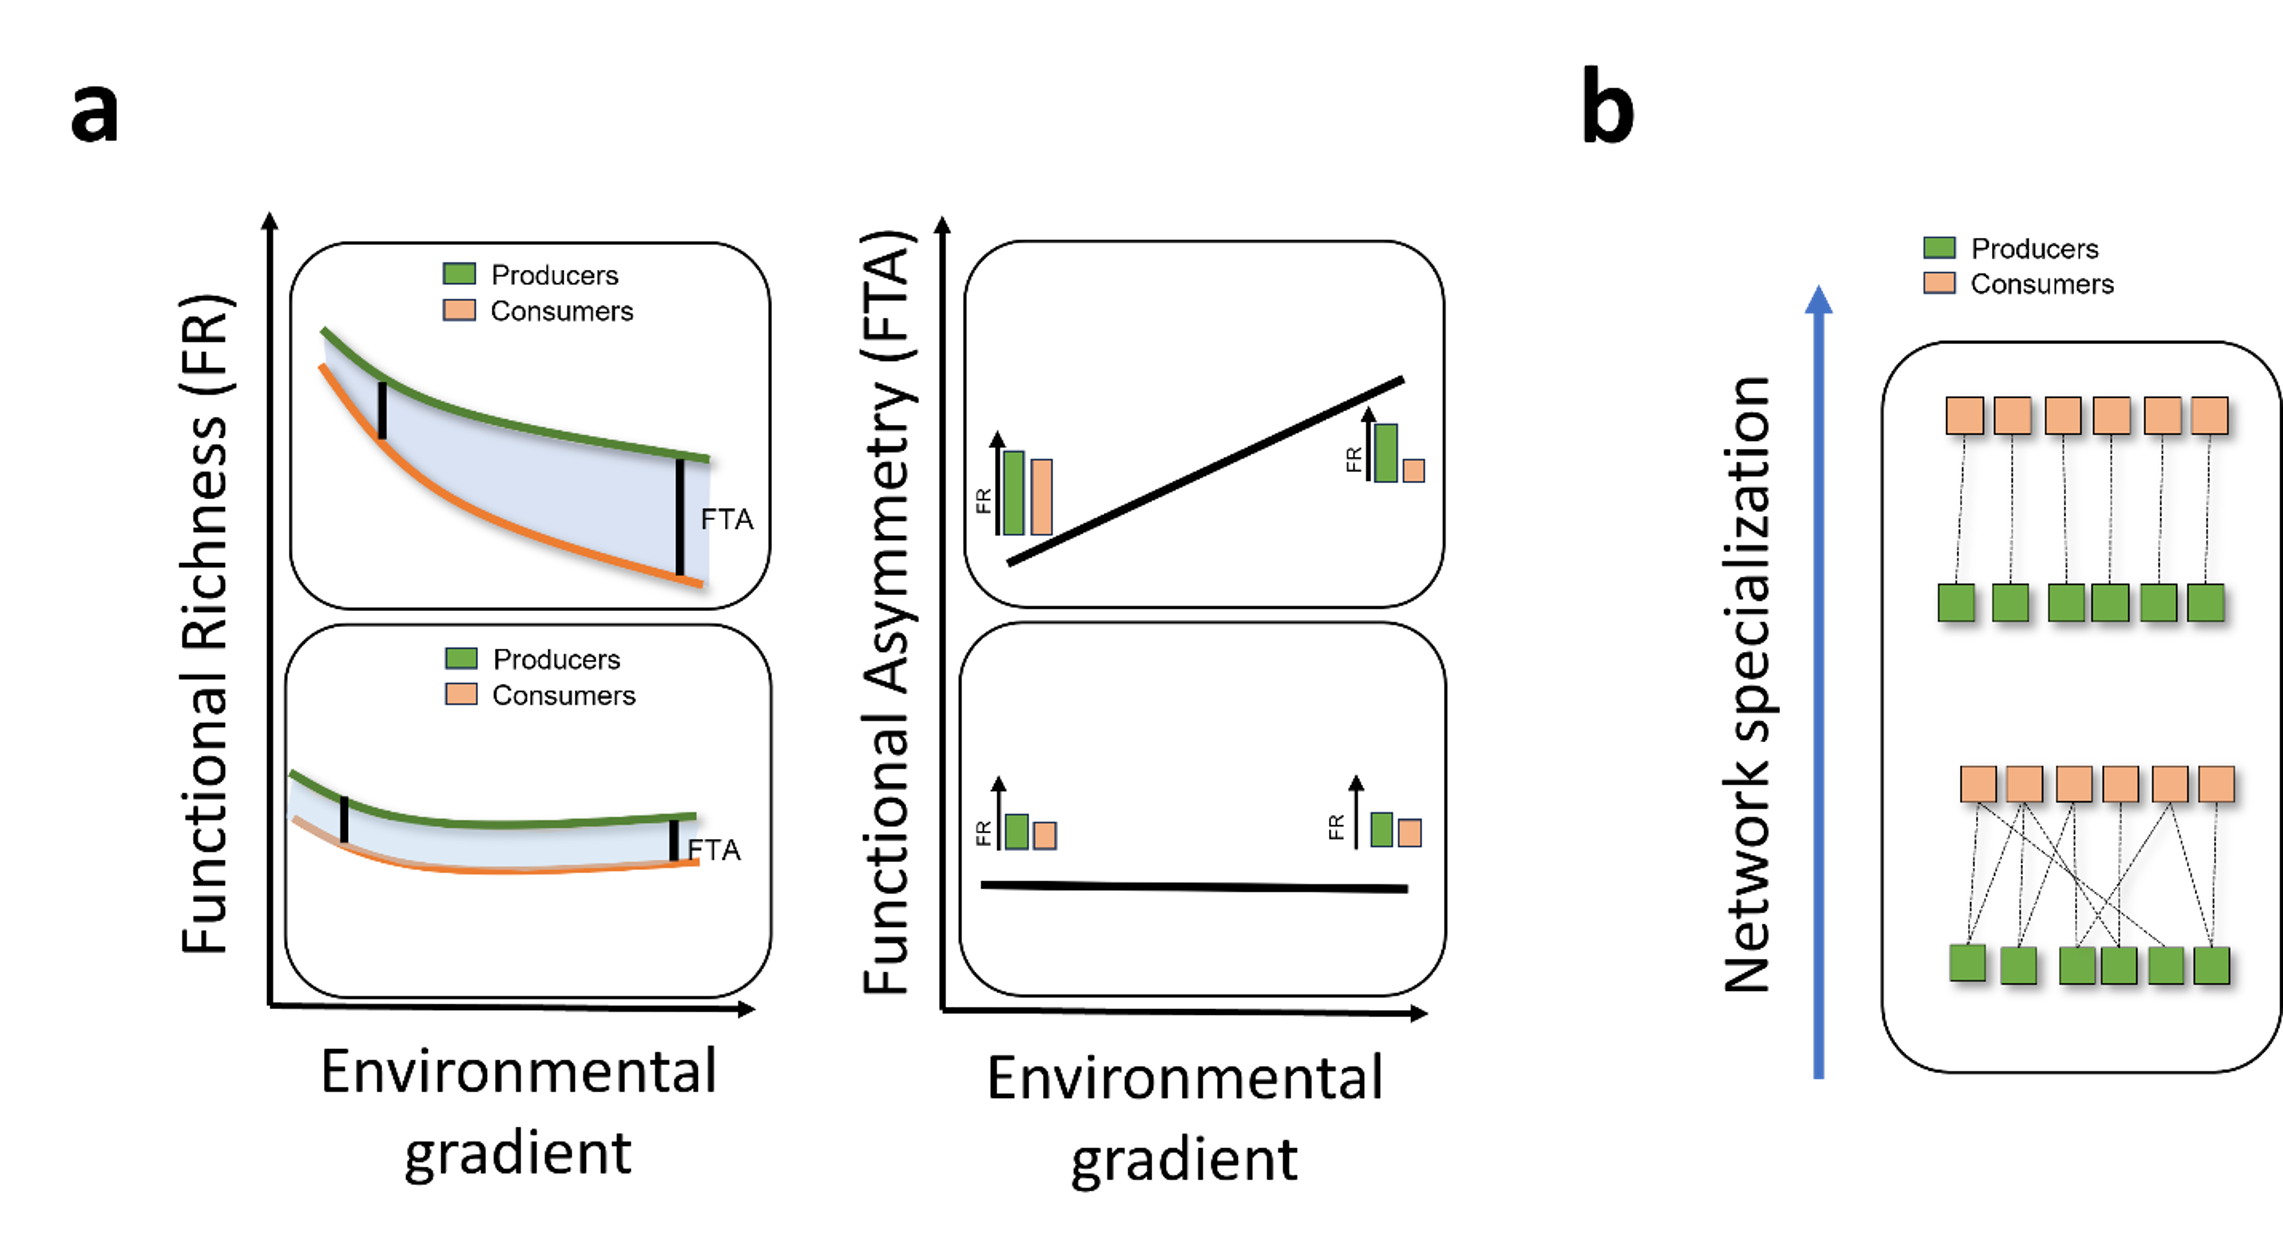
\includegraphics[width=5.20833in,height=\textheight,keepaspectratio]{images/00_Figure01.png}

}

\caption{\label{fig-01}This conceptual model illustrates the dynamic
relationship between functional diversity metrics---specifically
Functional Richness (FR) and Functional Trait Asymmetry (FTA)---and
environmental gradients within ecological networks. The left panel of
Figure a) visualizes the variation in FR for producers (depicted in
green) and consumers (depicted in orange) along an environmental
gradient. As the environmental gradient intensifies (e.g., through
changes in temperature, precipitation, or habitat fragmentation), FR for
both producers and consumers generally decline. However, this decline
can occur at different rates, leading to two scenarios: (1) Differential
Decline in FR: If consumer FR declines more sharply than producer FR, a
substantial increase in Functional Trait Asymmetry (FTA) occurs. (2)
Parallel Decline in FR: Alternatively, if both producer and consumer FRs
decline at a similar rate, FTA remains relatively constant along the
gradient. This scenario indicates a balanced impact of environmental
changes across trophic levels, preserving the relative functional
relationship between producers and consumers. Figure b) shifts focus to
the implications of changing FTA on network specialization---a measure
of how distinct generalized interactions are between producers and
consumers within ecological networks.}

\end{figure}%

Frameworks linking multitrophic functional diversity to network topology
along broad-scale environmental gradients are crucial to understand the
effects of global change on biodiversity and ecosystem function (Bello
et al., 2023; Dehling et al., 2021; Schleuning et al., 2012). Functional
responses of consumer and producer assemblages to climate influence
functional richness at the level of the multitrophic community (Garcı́a
et al., 2018). Because some of these traits are involved in interactions
across trophic levels, the filtering of traits along environmental
gradients could constrain the identity, number, and frequency of species
interactions and therefore, network topology (Albrecht et al., 2018;
Emer \& Memmott, 2023; Marjakangas et al., 2022). As an example,
constraints of varying intensities along climatic gradients, which limit
the relative availability of interaction partners across trophic levels,
could influence emergent patterns in network structure such as the
specialization of multispecies interactions (Blüthgen et al., 2006,
2007; Marjakangas et al., 2022). While high levels of network
specialization represent networks predominantly made of ``one-to-one''
interactions, low levels of network specialization represent networks
with species showing predominantly ``one-to-many'' interactions
(Blüthgen et al., 2006; Blüthgen \& Klein, 2011)
\hyperref[fig-01]{(Figure 1B)}. One highly expected outcome is that when
functional trophic asymmetry is high, networks will have low
specialization. For example, take a plant community exhibiting a low
richness of flower displays and which is associated with a bee community
(pollinators) exhibiting a wide variety of proboscis lengths. These
plants are unlikely to form ``one-to-one'' interactions with only a
subset of bee species that have matching proboscis length. Otherwise,
non-matching pollinators would have no food resources and be extirpated.
By partitioning deviations from expected FTA and network specialization
relationships with null models, one can separate the relative influences
of processes operating between trophic levels (e.g.~trait matching) and
those within trophic levels (e.g.~environmental selection) in network
assembly (Marjakangas et al., 2022). However, the relationship between
network specialization and functional trophic asymmetry has not been
fully explored.

Preserving mutualistic interactions between palms and their mammalian
frugivores is important to sustain biodiversity and ecosystem function
in the tropics (Bogoni et al., 2020; Marques Dracxler \& Kissling,
2022). Mammalian frugivores facilitate the dispersal of palm fruits,
which helps to prevent local extinctions amid disturbance and to
maintain biodiversity in these ecological networks (Acevedo-Quintero et
al., 2020; Dehling et al., 2022; Messeder et al., 2021). To effectively
preserve these interactions, it is crucial to understand how
co-occurring palm (producer) and mammalian frugivore (consumer)
communities respond to environmental gradients. By examining
co-variation in their functional richness across broad geographic scales
and linking those patterns to spatial and/or temporal variation in
climate, we can identify key abiotic factors that influence the assembly
of their mutualistic relationships. Here, we ask (1) \emph{which
climatic variable(s) best explains geographic variation in the
functional richness of palms and mammal frugivores}, (2) \emph{whether
differences in these relationships lead to functional trophic asymmetry
(hereafter FTA)}, and (3) \emph{which climatic variable best explains
geographic variation in FTA across the Neotropics}. We also ask (4)
\emph{whether the strength of interactions between palm-frugivore
interaction guilds relates to the strength of the relationship between
FTA and climate}. Finally, we ask (5) \emph{whether geographic variation
in FTA relates to network specialization}.

\subsection{Methods}\label{methods}

\subsubsection{Study system}\label{study-system}

We focused on multitrophic communities of Neotropical palms and their
mutualistic, seed dispersing, mammalian frugivores Figure~\ref{fig-02}.
Palms (Plantae:Arecaceae) are a keystone plant family in tropical
regions that provides fruit resources to a wide variety of vertebrate
frugivores, including birds and mammals (Muñoz et al., 2019). Frugivore
mammals (Animalia:Mammalia) are among the most important palm-seed
dispersers, particularly over long distances. Most frugivore mammals
feeding on palms are seed eaters and pulp eaters, dispersing palm seeds
mostly via ectozoochorus dispersal (Messeder et al., 2021). Importantly,
frugivory-related traits have notably underlain palm diversification and
played a key role in the evolution of palm traits (Kissling et al.,
2012; Onstein et al., 2014, 2017).

\subsubsection{Data sources}\label{data-sources}

\paragraph{Geographic distribution
data}\label{geographic-distribution-data}

We obtained binary species distribution data (present/absent) on palms
from the geographic range maps of (Bjorholm et al., 2005) and on mammals
from the IUCN (International Union for the Conservation of Nature) data
portal. To generate local gridded multitrophic species assemblages
across the Neotropics, we intersected the species-level range maps with
a spatial grid where each grid cell represented every 1 by 1 degree
latitude and longitude change along the extent of the entire Neotropics.
We then listed all palm and mammal frugivore species co-occurring in
each grid-cell as our grid-cell level multitrophic assemblage.

\paragraph{Trait data}\label{trait-data}

We collected species-level multitrophic trait data related to the
physiological tolerance of palms and frugivorous mammals to the abiotic
environment and to their mutualistic interactions. For palms, we
extracted data from the PalmTraits 1.0 dataset (Kissling et al., 2019).
We collected data on growth form, maximum stem height, and average fruit
length. For frugivorous mammals, we obtained trait data from the
EltonTraits 1.0 database (Wilman et al., 2014). We selected data on body
mass, diet, and daily activities. Diet data from the EltonTraits 1.0
database is coded as percentage use distribution across ten diet
categories. We excluded from our analysis species without fruit in their
diet. Activity was coded as a dummy variable with three categories
(Diurnal, Crepuscular, Nocturnal). Finally, body mass was coded as a
numerical variable in kg. We excluded bats from the analysis as almost
no Neotropical bat species is feeding on palm fruits (Messeder et al.,
2021). From this dataset, we selected only those species whose range in
gridded multitrophic communities within a regular 1×1° latitude grid
co-occur with at least 5 other palm and mammal frugivore species in the
same grid. In total, we worked with a subset from this dataset of 494
palm species and 488 mammal frugivore species with linked trait and
geographic data. Pairwise interaction data

We used data on seed dispersal interactions between palms and mammals
for the Neotropics, originating from recollections of seed dispersal
records found in the published literature and interaction records are
recorded at the species level (Muñoz et al., 2019). Each pairwise
species interaction record reflects where an article mentions the fruit
or the seed of a palm being dispersed, carried or defecated by a
frugivorous mammal. Interaction records collected in this database were
previously vetted to reflect effective seed dispersal interactions,
while avoiding those that reflect mere seed consumption (vetting
criteria found in: Muñoz et al. (2019) ). In total, we gathered a total
of 581 interaction records between 69 palms and 111 frugivore mammals.

\paragraph{Environmental data}\label{environmental-data}

We used bioclimatic variables from WorldClim (Fick \& Hijmans, 2017) to
represent large-scale spatial and temporal variation of climate in the
Neotropics. Specifically, we used mean annual temperature (BIO01), total
annual precipitation (BIO12), temperature seasonality (BIO04) and
precipitation seasonality (BIO15). Using a moving window, we compute
simple averages for every set of bioclimatic records at each grid cell,
thereby re-scaling the spatial resolution of bioclimatic variables to 1
by 1 degree grid resolution from their original resolution (1 x 1 km2)
to match the spatial resolution of our grid cell species-level data
Figure~\ref{fig-02}

\begin{figure}

\centering{

\pandocbounded{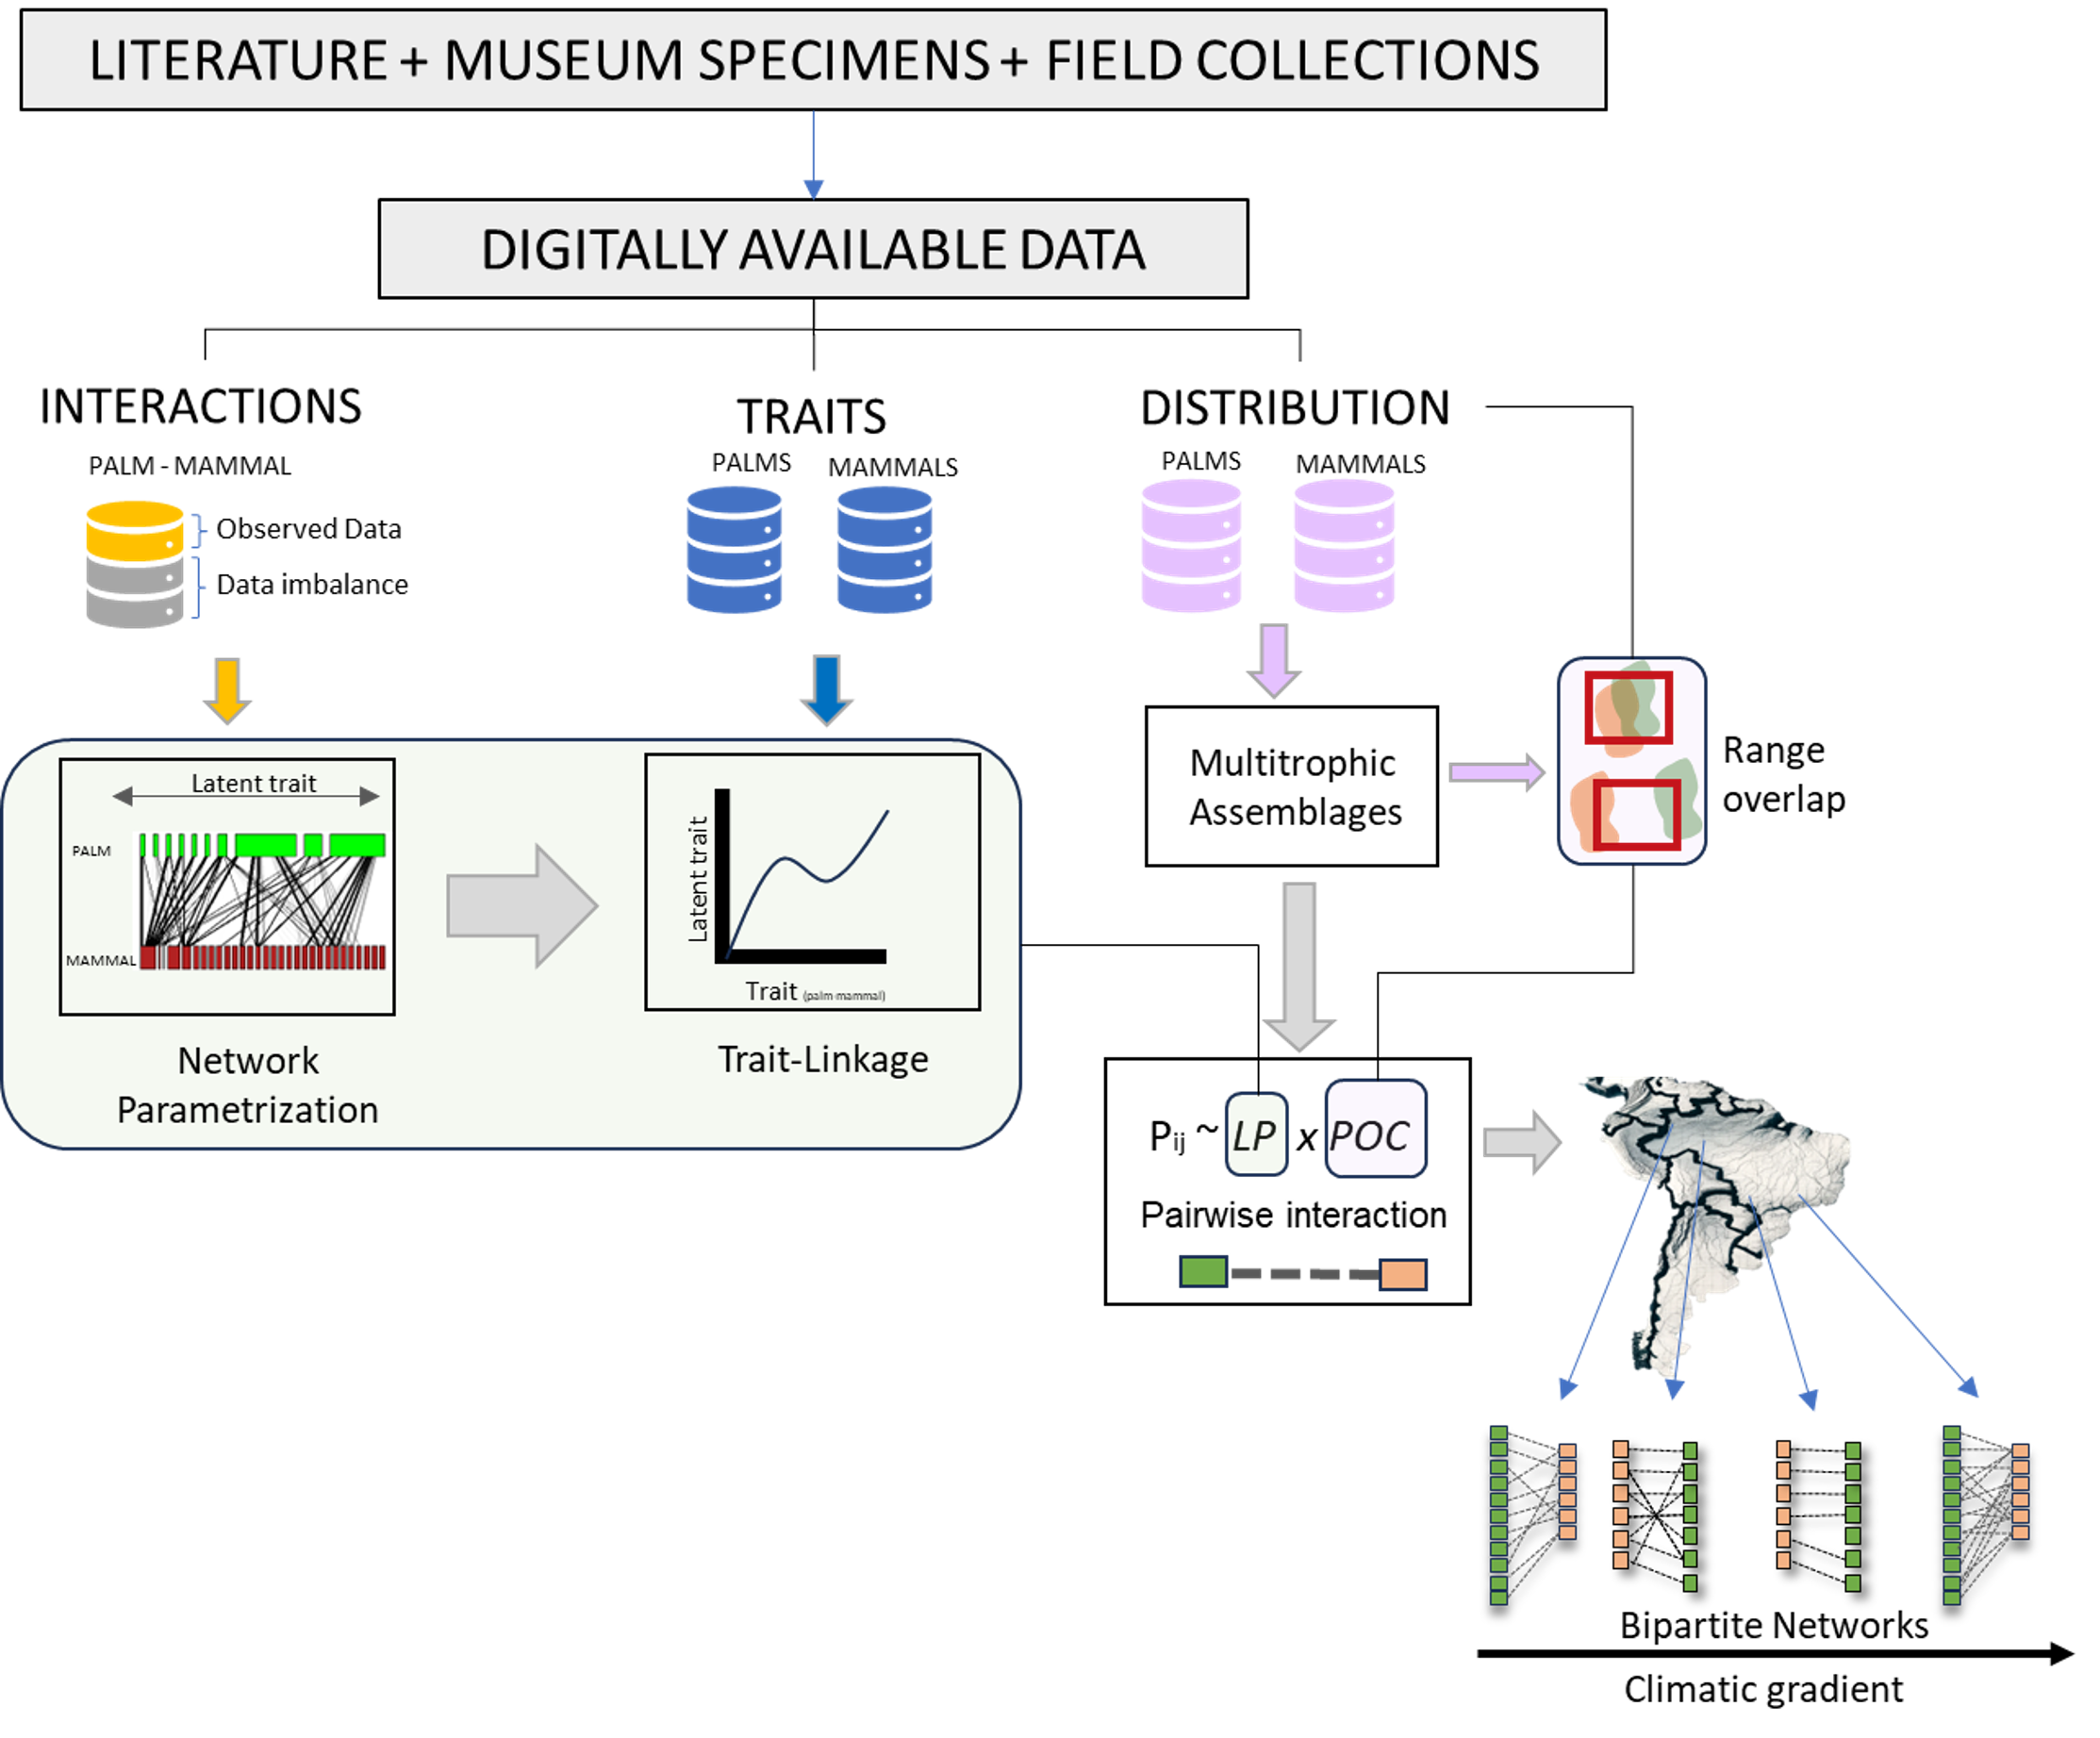
\includegraphics[keepaspectratio]{images/00_Figure02.png}}

}

\caption{\label{fig-02}Workflow illustrating the integration of
ecological and trait data from digital sources to model species
interactions and predict ecological networks across geographic regions.
The figure illustrates a workflow for integrating ecological interaction
data derived from literature, museum specimens, and field collections
into digitally available datasets. These datasets are used to build
ecological network models and link species interactions to their
biological traits. The approach involves parameterizing networks based
on latent traits and identifying trait-linkages, which are subsequently
utilized to predict ecological interactions and networks across
different geographic locations (e.g.~The Neotropics)}

\end{figure}%

\subsubsection{Statistical analysis}\label{statistical-analysis}

Building a probabilistic continental metaweb from aggregated binary
interaction records Here, we fitted latent variable network structural
models that vary in their assumptions to estimate interaction
probabilities from observed binary data on species interactions. (Figure
3) Specifically, we tested: the stochastic block model (SBM), the
connectance model, the trait-matching model, and the matching-centrality
model (Terry \& Lewis, 2020). The SBM assumes that ecological networks
are modular, with species of consumers interacting more within their
preferred groups of producers (i.e., interaction guilds). This model
outputs three incidence matrices, reflecting predicted interactions: (i)
one with guilds of palm species based on their modular interactions with
mammals, (ii) a similar one for mammals, and (iii) one representing the
interaction probabilities (Theta) among the guilds of each group (i.e.,
palm guilds-mammal-guild). The connectance model posits that
interactions of specialist species are subsets of those of generalist
species, optimizing connectivity scores to recreate observed network
patterns. The trait-matching model assumes non-random species
interactions determined by trait differences, optimizing parameters
along latent-trait axes. The matching-centrality model combines
connectivity scores and latent-trait axes (Terry and Lewis 2020). We
fitted these models to our available interaction data and selected the
model that best predicted the observed continental pattern of seed
dispersal interactions. Using Youden's J as a metric that balanced model
sensitivity and specificity (Poisot, 2023), we found that the SBM was
the best supported model Figure~\ref{fig-03} and therefore focused on it
in the rest of the manuscript. Additional details about the model
assumptions are explained in Supplementary Text S1.

\begin{figure}

\centering{

\pandocbounded{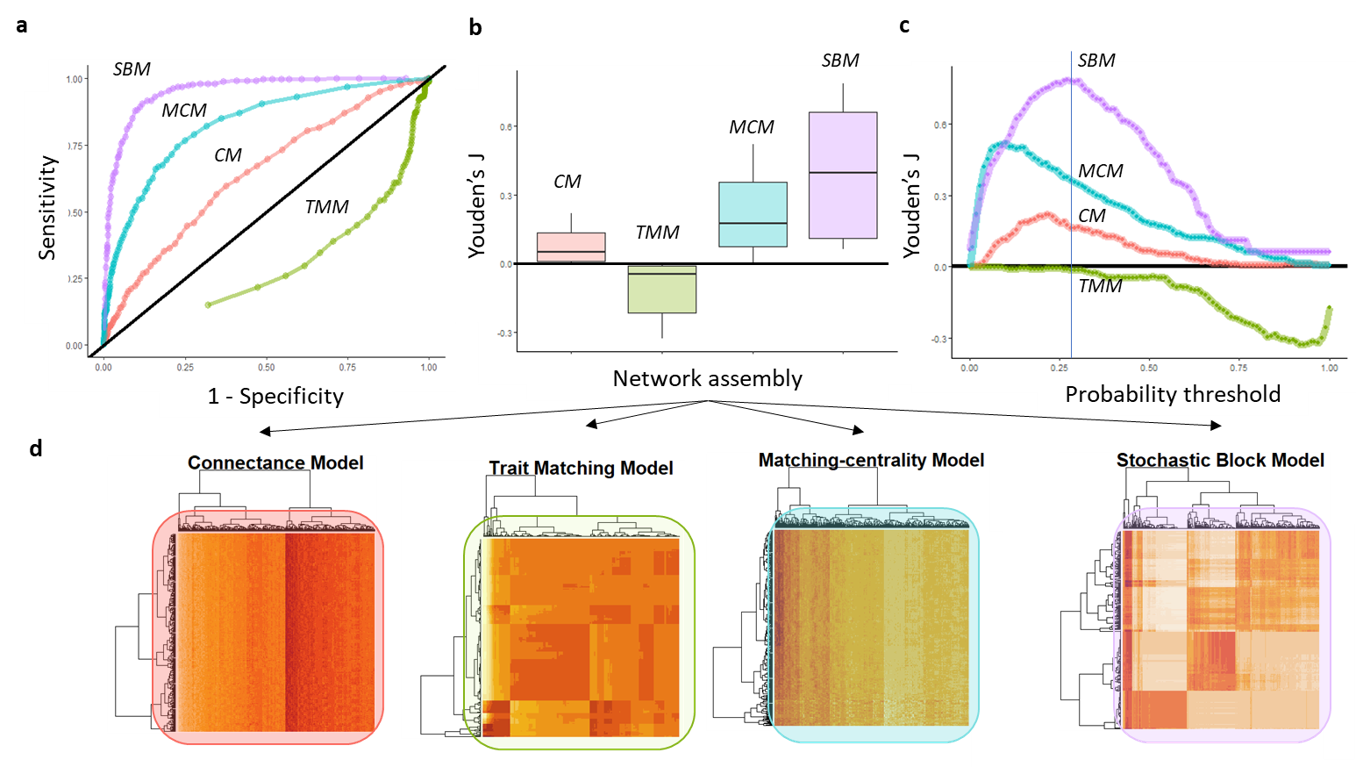
\includegraphics[keepaspectratio]{images/00_Figure03.png}}

}

\caption{\label{fig-03}Model evaluation plots of distinct structural
models fitted to predict the structure of the observed palm-mammal
frugivore interactions in the Neotropics. In this figure we illustrate a
comparison of ecological network assembly models using ROC curves (a),
Youden's J index (b,c), and clustering heatmaps (d) to illustrate
differences in predicting species interactions. Specifically, the figure
compares four ecological network assembly models---Centrality Model
(CM), Trait Matching Model (TMM), Matching Centrality Model (MCM), and
Stochastic Block Model (SBM)---in their ability to accurately predict a
observed binary pattern of species interactions. For our study, this
observed pattern reflected the incidence of seed dispersal interactions
between palms and their mammalian frugivores. The ROC curves (a)
indicate model performance in terms of model sensitivity (i.e.~true
positive rate) versus model specificity (true negative rate). Curves
further above the diagonal demonstrate stronger predictive ability,
showing that the model performs significantly better than random
guessing in identifying ecological interactions. If a ROC curve is close
to or below this diagonal, the model's predictive performance is no
better than random chance. The central boxplot summarizes the Youden's J
index, where higher values reflect higher overall predictive accuracy.
Panel (c) shows Youden's J index variation over different probability
thresholds to materialize binary interactions. The heatmaps below
visualize clustering patterns, highlighting structural differences in
predicted interaction networks for each model.}

\end{figure}%

\paragraph{Identifying interaction
guilds}\label{identifying-interaction-guilds}

Since the hyperparameters of the Stochastic Block Model (SBM) provided
the best fit for capturing the observed interactions, palm-frugivore
interaction networks are highly modular and certain groups of producers
are more likely to interact with certain groups of consumers than
others, and vice versa. In this context, we define an interaction guild
as a distinct group of palm and mammal species within the continental
metaweb that exhibits similar interaction patterns. Within each guild,
both producer and resource species perform comparable functional roles
in the network. Within and between each guild combination of consumers
and producers, species pairs exhibit the same interaction strength,
where interaction strength is defined as the magnitude or intensity of
the effect that one species has on another within an ecological network.
Here we estimate interaction strength as the probability that a species
pair would interact in nature. The SBM estimates such interaction
probabilities based on the frequency of interactions observed between
species assigned to given guild of consumer or producer. The SBM model
uses maximum likelihood to adjust the number of guilds and the
distribution of interaction probabilities within and between guilds such
that they best explain the observed pattern of interactions. Using SBMs
largely reduces the complexity of dealing with interaction strengths by
treating them as a guild-level phenomenon instead of a species-specific
one.

\paragraph{Downscaling the continental metaweb to generate grid-cell
level
networks}\label{downscaling-the-continental-metaweb-to-generate-grid-cell-level-networks}

The digital availability of primary biodiversity data on palms and their
mammalian frugivores was imbalanced, with a high availability of
distribution ranges and species traits, but a limited number of
interaction records. Therefore, to downscale our initial metaweb to
include interactions between every potentially co-occurring palm and
mammal frugivore in every grid cell across the Neotropics, we used a
twofold approach Figure~\ref{fig-02}.

First, we employed multinomial logistic regression models to predict the
species level SBM model results (i.e., interaction guild affiliation)
from species-level trait data. We justify the choice of multinomial
logistic regression models as these can handle the prediction of
non-binary outcomes, such as the labeling of interaction guilds per
species. We fitted separate multinomial models for palms and mammal
frugivores using a label backpropagation algorithm and a neural network
engine, with 75\% of the data allocated for training and the 25\%
remaining for testing. We use neural networks because they are useful
when dealing with multicollinearity, as they can learn complex and
non-linear relationships and interactions among multiple predictor
variables. This allowed us to separate the relative importance of
distinct matching traits on SBM group affiliations. We extracted
variable importance scores based on the combinations of the absolute
values of the best fit model weights (Gevrey et al., 2003)

Second, we considered local pairwise species interaction probabilities
as the product of the values from the Theta matrix from the SBM model
that represent the latent interaction probabilities between species
pairs within and between groups multiplied by their probability of
co-occurrence (POC) in a grid cell. To represent species' co-occurrence
probabilities, we used the reciprocal distance between the centroids of
species pair ranges within the grid-cell, divided by the sum of their
range areas within the grid-cell. This implied that within each grid
cell, species with closer range centroids and larger cumulative areas
are more likely to co-occur and interact. This approach allowed us to
recreate synthetic probabilistic plant-mammal frugivore networks for
each grid-cell across the Neotropics, while accounting for the
heterogeneity of species ranges within each grid.

\paragraph{Estimating Functional
Richness}\label{estimating-functional-richness}

We investigated the spatial variation in the relative distribution of
species counts of producers and consumers across all guilds in a grid
cell, as an interaction network-level indicator of the spatial
distribution of producer and consumer species' functional richness. We
estimated functional richness (FR) from the results of the SBM model
fit, specifically, from the matrices representing the interaction
guilds. Thus, to measure functional richness for each trophic level, we
calculated a grid-cell level vector representing the number of species
across all interaction guilds (n = 7). To account for the differences in
the total number of palm and mammal species across grid cells, we
normalized this vector to the total sum of palm or mammal species counts
within each grid cell.

\paragraph{Estimating Functional Trophic Asymmetry
(FTA)}\label{estimating-functional-trophic-asymmetry-fta}

We quantified functional trophic asymmetry (FTA) as the absolute
difference between the functional richness vectors across trophic
levels. Since each palm and mammal species in every grid cell had the
potential to be affiliated with any of the seven interaction guilds and
to interact with any species from the opposite trophic level both within
and between guilds, we derived one FTA measures for each grid cell, and
for each pairwise palm-mammal guild combination (Figure S2).

\paragraph{Estimating Network Specialization
(H2')}\label{estimating-network-specialization-h2}

We estimated network specialization for each grid cell using the metric
H2'. H2' is a network-level index that varies between 0 and 1 (Blüthgen
et al.~2007). High values indicate networks that are more specialized,
meaning that species from one trophic level interact with only or few
species in the opposite trophic level. Low H2' values indicate that
there is a low specificity of interactions in the network, meaning that
species from one trophic level interact with multiple species at the
other trophic level. Because inferred networks varied in their network
size (i.e., number of unique interactions between palms and mammals), we
rarefied the computation of H2' to networks for each grid cell such that
they would all have the same size (i.e., number of interactions).
Specifically, we rarefied all networks to 100 pairwise interactions and
repeated the procedure 999 times to get a distribution of rarefied H2'
values (Terry \& Lewis, 2020). We then selected the median of this H2'
distribution as our grid cell-level measure of network specialization.

\paragraph{Assessing the influence of climate on
FTA}\label{assessing-the-influence-of-climate-on-fta}

To assess whether climate has an influence on FTA, we fitted a
Generalized Additive Model (GAM) to examine the relationships between
FTA and four continuous bioclimatic predictors. The GAM approach allows
for modelling flexible non-linear relationships between the predictors
and the response variable using smoothed functions (Wood, 2017). The
predictor variables included in our models were Mean annual temperature
(Temp), Total annual precipitation (Prec), Temperature seasonality (TS),
and Precipitation seasonality (PS). Collectively, are these climatic
factors known contemporary factors influencing both the regional and
global diversity of plants and mammals (Holt et al., 2018). We fitted
separate splines for each of the climatic predictors.

Assessing how interaction strength mediates the influence of climate on
FTA To assess whether the strength of interaction between producer and
consumer guilds mediate the strength of the relationship between FTA and
climate, we included interaction strength as an interaction term in the
GAM, allowing splines between FTA and climate to vary non-linearly
depending on interaction strength.

\paragraph{Assessing the relationship between FTA and
H2'}\label{assessing-the-relationship-between-fta-and-h2}

We used Generalized Additive Model (GAM) to investigate the relationship
between rarefied grid cell network level specialization (H2') as a
response variable and FTA (z-scores) as the main predictor. We also
added the effect of Mean annual temperature, Total annual precipitation,
Precipitation seasonality, and Temperature seasonality as covariate
functions because these climate variables may influence H2'
independently of FTA, allowing us to isolate the specific impact of FTA
on H2' while controlling for the indirect effects of climate on FTA.
Here, we estimated grid-cell level functional trophic asymmetry (FTA')
by summing the FTA values across all interaction guilds, weighted by
their respective interaction strengths. This approach was selected as
accounts for the uneven contributions of each guild to network
structure, highlighting whether changes in network specialization are
primarily driven by shifts in FTA within the more specialized
interaction guilds.

\subsection{Results}\label{results}

\subsubsection{Interaction guild
delineation}\label{interaction-guild-delineation}

The Theta matrix derived from the SBM (Stochastic Block Model) analysis
Figure~\ref{fig-04} reflects the modular pattern assumed by this model,
here identified as the best for frugivore-mammal interactions.
Therefore, these interactions are stronger within rather than between
guild pairs. Given the associations found with the theta matrix, we can
derive that the following high-level trait-trait associations: a) Tall
palms with medium-sized fruits can associate strongly with small to
medium sized mammals that consume moderate to high amounts of fruit. b)
Acaulescent or small-stemmed palms with small to large fruits correlate
strongly with either small, moderately frugivorous mammals or small
mammals with relatively low frugivory. Finally, c) medium-sized to large
sized mammals with moderate to low frugivory levels interact with
species with intermediate palm traits (e.g., moderately tall erect palms
with medium-sized fruits) (Figure S1).

\begin{figure}

\centering{

\pandocbounded{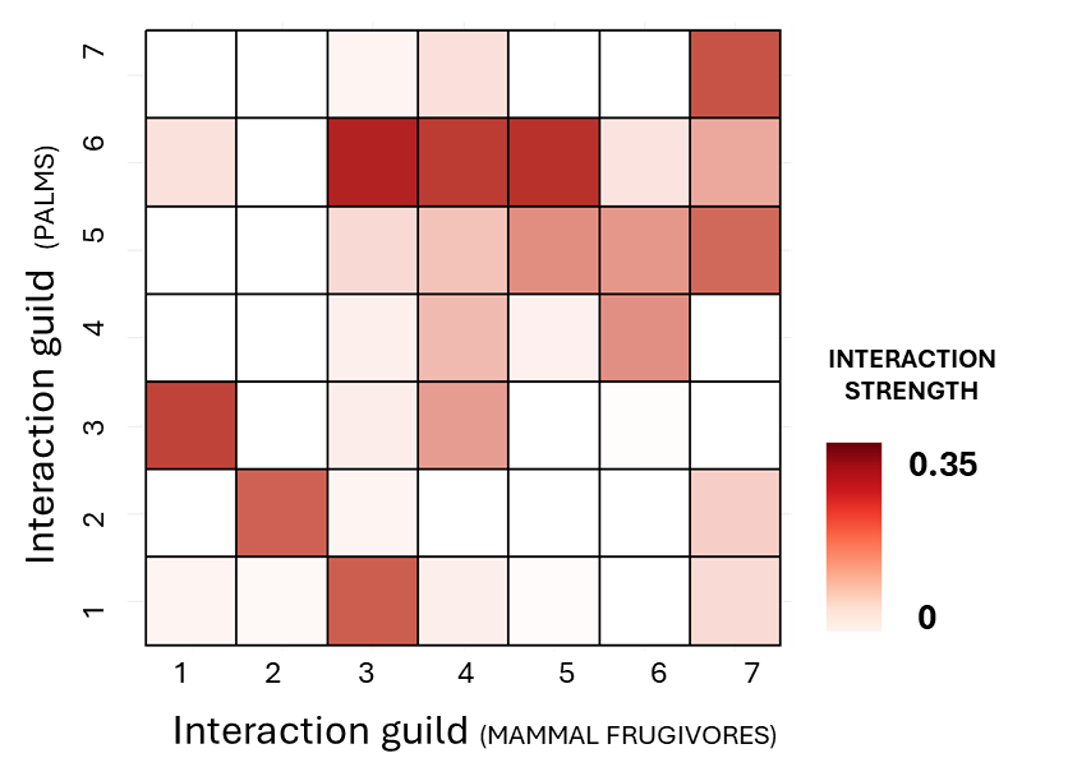
\includegraphics[keepaspectratio]{images/00_Figure04.png}}

}

\caption{\label{fig-04}Heatmap depicting the probability of interaction
between palm and mammal interaction guilds defined as blocks by the
Stochastic Block Model (SBM). The intensity of red shading correlates
with the strength of these interactions, where darker shades signify
higher probabilities of interaction between species within or between
interaction guilds (SBM blocks), where the probability was inferred
using the Stochastic Block Model's estimated interaction parameters
(theta Matrix) derived from fitting the model to observed binary
(presence = 1, absence = 0) interaction data compiled from scientific
literature.}

\end{figure}%

\subsubsection{The influence of climate on functional
richness}\label{the-influence-of-climate-on-functional-richness}

At the grid-cell level, when ignoring interaction guild affiliations,
neither the functional richness of palms or mammals relates to
geographic variation in climate (Figure S3,S4, Table S1,S2). The
functional richness of palms does not relate to temperature (F = 3.00, P
\textless{} 0.05), precipitation (F = 1.19, P = 0.23), temperature
seasonality (F = -0.27, P = 0.79) or precipitation seasonality (F =
0.68, P = 0.50). The functional richness of mammals positively relates
to mean annual temperature (F = 10.60, P \textless{} 0.05) but not to
precipitation (F = 0.001, P = 1.00), temperature seasonality (F = 0.52,
P = 0.60) or precipitation seasonality (F = 1.67, P = 0.10). When
considering guild affiliation in our analyses, there are marked
differences in the relationship between functional richness and climate
among trophic levels \hyperref[fig04]{(Figures 4a,4b)}. The functional
richness of palm positively relates to precipitation seasonality for
guilds 5 (F = 5.62, P \textless{} 0.01) and negatively relates to
precipitation seasonality for guild 6 (F = 8.37, P = 0.01) (Figure S3).
In contrast, the relationship between the functional richness of mammals
and precipitation seasonality does not vary among guilds. However, the
relationship with temperature does vary among guilds. Specifically, the
functional richness of guild 3 positively relates to temperature (F =
11.21, P \textless{} 0.01) whereas that of other guilds does not relate
to temperature (Figure S4).

\begin{tcolorbox}[enhanced jigsaw, colframe=quarto-callout-color-frame, opacityback=0, bottomrule=.15mm, left=2mm, toprule=.15mm, arc=.35mm, rightrule=.15mm, colback=white, breakable, leftrule=.75mm]

\vspace{-3mm}\textbf{Table 1}\vspace{3mm}

\textsubscript{Source:
\href{https://lessardlab.github.io/fta_ec_networks/index-preview.html}{Article
Notebook}}

\begin{longtable*}{ccccc}
\caption*{
{\large \textbf{Parametric coefficients}}
} \\ 
\toprule
 & Estimate & Std. Error & t value & p-value \\ 
\midrule\addlinespace[2.5pt]
\cellcolor[HTML]{D9D9D9}{Intercept} & \cellcolor[HTML]{D9D9D9}{0.21} & \cellcolor[HTML]{D9D9D9}{0} & \cellcolor[HTML]{D9D9D9}{271.5} & \cellcolor[HTML]{D9D9D9}{\textbf{>0.001 ***}} \\ 
\bottomrule
\end{longtable*}

\textsubscript{Source:
\href{https://lessardlab.github.io/fta_ec_networks/index-preview.html}{Article
Notebook}}

\begin{longtable*}{ccccc}
\caption*{
{\large \textbf{Smooth Terms}}
} \\ 
\toprule
 & edf & Ref.df & F & p-value \\ 
\midrule\addlinespace[2.5pt]
\cellcolor[HTML]{D9D9D9}{Mean Annual Temperature} & \cellcolor[HTML]{D9D9D9}{1.00} & \cellcolor[HTML]{D9D9D9}{1} & \cellcolor[HTML]{D9D9D9}{5.97} & \cellcolor[HTML]{D9D9D9}{\textbf{0.01 *}} \\ 
\cellcolor[HTML]{D9D9D9}{Mean Annual Temperature x interaction strength} & \cellcolor[HTML]{D9D9D9}{0.00} & \cellcolor[HTML]{D9D9D9}{27} & \cellcolor[HTML]{D9D9D9}{0.00} & \cellcolor[HTML]{D9D9D9}{\textbf{0.57}} \\ 
\cellcolor[HTML]{D9D9D9}{Precipitation seasonality} & \cellcolor[HTML]{D9D9D9}{1.00} & \cellcolor[HTML]{D9D9D9}{1} & \cellcolor[HTML]{D9D9D9}{0.30} & \cellcolor[HTML]{D9D9D9}{\textbf{0.59}} \\ 
\cellcolor[HTML]{D9D9D9}{Precipitation seasonality x interaction strength} & \cellcolor[HTML]{D9D9D9}{1.67} & \cellcolor[HTML]{D9D9D9}{27} & \cellcolor[HTML]{D9D9D9}{0.14} & \cellcolor[HTML]{D9D9D9}{\textbf{0.05.}} \\ 
\cellcolor[HTML]{D9D9D9}{Temperature seasonality} & \cellcolor[HTML]{D9D9D9}{1.00} & \cellcolor[HTML]{D9D9D9}{1} & \cellcolor[HTML]{D9D9D9}{0.19} & \cellcolor[HTML]{D9D9D9}{\textbf{0.67}} \\ 
\cellcolor[HTML]{D9D9D9}{Temperature seasonality x interaction strength} & \cellcolor[HTML]{D9D9D9}{0.00} & \cellcolor[HTML]{D9D9D9}{27} & \cellcolor[HTML]{D9D9D9}{0.00} & \cellcolor[HTML]{D9D9D9}{\textbf{0.54}} \\ 
\cellcolor[HTML]{D9D9D9}{Total Annual Precipitation} & \cellcolor[HTML]{D9D9D9}{1.00} & \cellcolor[HTML]{D9D9D9}{1} & \cellcolor[HTML]{D9D9D9}{0.28} & \cellcolor[HTML]{D9D9D9}{\textbf{0.60}} \\ 
\cellcolor[HTML]{D9D9D9}{Total Annual Precipitation x interaction strength} & \cellcolor[HTML]{D9D9D9}{0.00} & \cellcolor[HTML]{D9D9D9}{27} & \cellcolor[HTML]{D9D9D9}{0.00} & \cellcolor[HTML]{D9D9D9}{\textbf{0.47}} \\ 
\cellcolor[HTML]{D9D9D9}{Interaction strength} & \cellcolor[HTML]{D9D9D9}{5.00} & \cellcolor[HTML]{D9D9D9}{5} & \cellcolor[HTML]{D9D9D9}{746.20} & \cellcolor[HTML]{D9D9D9}{\textbf{>0.001 ***}} \\ 
\bottomrule
\end{longtable*}

\textsubscript{Source:
\href{https://lessardlab.github.io/fta_ec_networks/index-preview.html}{Article
Notebook}}

\end{tcolorbox}

\subsubsection{The influence of climate on
FTA}\label{the-influence-of-climate-on-fta}

The distribution of functional trophic asymmetry (FTA) exhibited a
bi-modal pattern, with a primary cluster centered around local maxima of
FTA = 0.09 and a secondary cluster near a second local maxima of FTA =
0.49. A similar clustering pattern after standardizing FTA by the
strength of interaction guilds, however, the cluster of low FTA values
due to low or minimal interaction strength is more apparent
\hyperref[fig04]{(Figures 4c, 4d)}. The distribution of FTA varies
significantly across interaction guilds (Figure S5) The maximum FTA
record across all guilds was 0.93. Within individual guilds, the highest
FTA values were associated with interactions between tall, erect palms
bearing medium to large fruits (guild 3) and highly frugivorous mammals
(guild 1) (Figure S5). Similarly, medium-sized palms with small to
medium fruits (guild 5) interact with large mammals exhibiting low
levels of frugivory (guild 6) also contributed significantly to high FTA
standardized values In contrast, interactions involving acaulescent or
short-stemmed palms with medium-sized fruits (guild 6) and small mammals
with limited frugivory intake (guild 3) consistently yielded the lowest
FTA standardized values (Figure S5) When ignoring interaction guilds,
functional trophic asymmetry (FTA) is positively related to mean annual
temperature (F = 5.97, P = 0.01). FTA is not related to precipitation (F
= 0.28, P = 0.13), precipitation seasonality (F = 0.30, P = 0.59) or
temperature seasonality (F = 0.19, P = 0.67) (Table 1). When considering
interaction guild affiliation in our analyses, there are marked
differences in how temperature (Temp) and Precipitation seasonality (PS)
interact among distinct interaction guild combinations
Figure~\ref{fig-05}. Specifically, an increase in the relative richness
of frugivores with low levels of fruit in their diet (i.e.~mammal
interaction guilds 3, 6 and 7) with increasing Temperature drove changes
in FTA along the temperature gradient \hyperref[fig-05]{(Figure 5a,
5c)}, while along increasing precipitation seasonality, FTA was driven
by the reduction in the richness of short palms with low to medium fruit
sizes (guild 5) and of tall palms with low fruit sizes (guild 2),
coupled with an increase in the relative richness of short stemmed and
acaulescent palms with medium to large fruits (guild 6) across the
climatic gradient \hyperref[fig-05]{(Figure 5b,5d)}.

\begin{figure}

\centering{

\pandocbounded{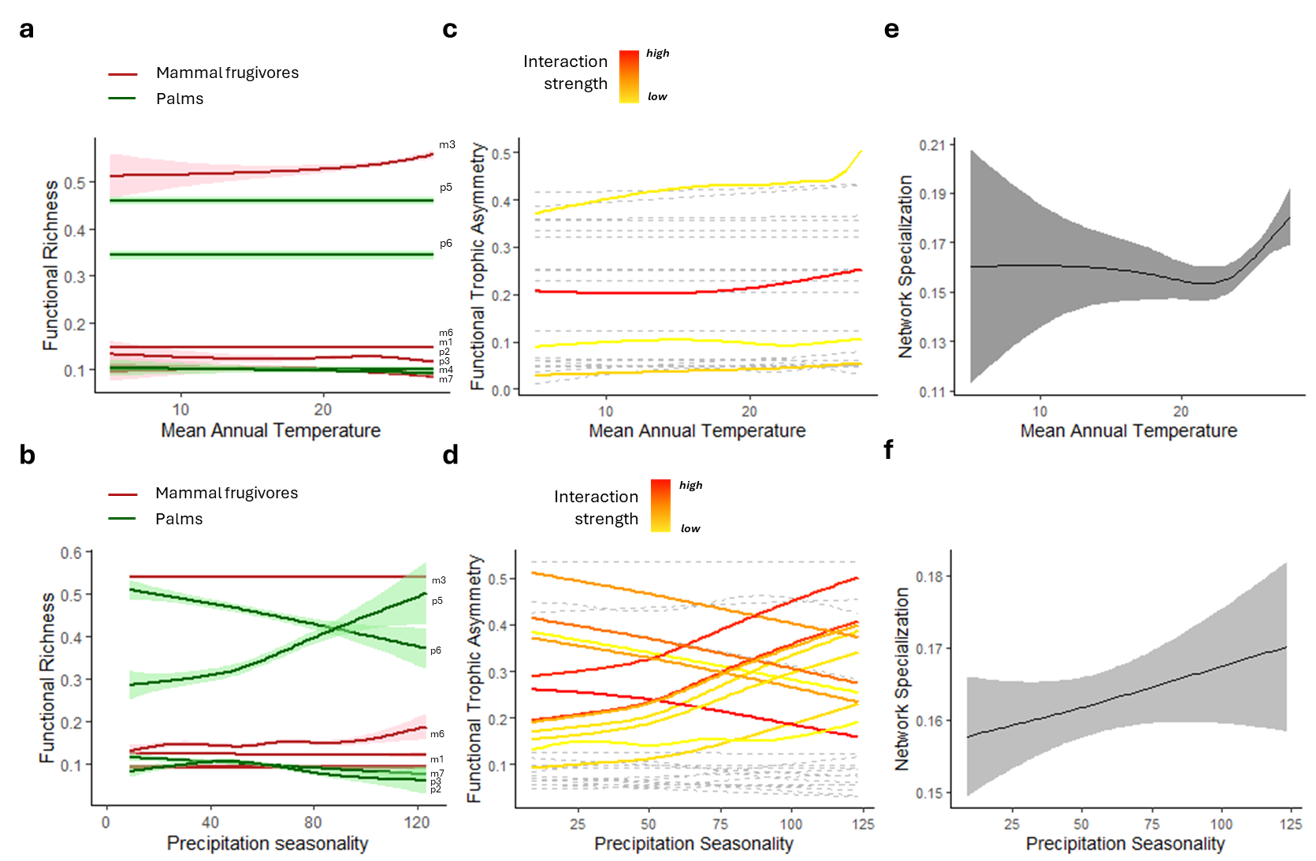
\includegraphics[keepaspectratio]{images/00_Figure05.png}}

}

\caption{\label{fig-05}Relationships between environmental gradients,
functional diversity, and network properties in the multitrophic system
of mutualistic palm-mammal frugivore networks in Neotropics. (a, b)
Trends in the functional richness of palms (green) and mammals (red) as
a function of mean annual temperature (a) and precipitation seasonality
(b), with shaded areas representing confidence intervals. Each trendline
estimates the change in Functional Richness of an interaction guild.
Each interaction guild corresponds to the species groupings found with
the Stochastic Block Model and it is identified with labels at the
higher end of the climatic gradient. (c, d) Functional trophic asymmetry
(FTA) across temperature (c) and precipitation seasonality (d) for all
combinations of potential interactions among and within guilds.
Interaction strength indicated by a color gradient from yellow (low) to
red (high). Trendlines for interaction guild combinations which are
significantly affected with the changes in the climatic gradient are
colored and shown in continuous lines. Trendlines for interaction guild
combinations which are not responsive to climate are shown in gray and
stippled lines. (e, f) Network specialization (z-score) along gradients
of mean annual temperature (e) and precipitation seasonality (f), with
shaded areas denoting confidence intervals. Network specialization is
measured with the specialization index (H'), rarefied to be measured in
networks of the same number of interactions, and z-score standardized
for networks across sites by using a null model that simulates
stochastic multispecies assembly.}

\end{figure}%

\subsubsection{Does interaction strength mediates the influence of
climate on
FTA?}\label{does-interaction-strength-mediates-the-influence-of-climate-on-fta}

The strength of interaction between guilds of consumers and producers
had an overall positive effect on FTA (Figure S6). FTA values showed a
bi-modal distribution with peaks at high and low ends of the interaction
strength spectrum. However, we did not find strong evidence supporting
that the relationship between FTA and climate depends on the strength of
interaction between interaction guilds (F = 746, P \textgreater{} 0.05).
The interaction term between guild interaction strength and
precipitation seasonality had a marginally significant, and positive,
effect on FTA. (F = 0.14, P = 0.051) (Table 1). Assessing the
relationship between FTA' and H2' We found that palm-mammalian frugivore
networks have moderate levels of trophic specialization (H2') ranging
from 0.12 to 0.25, where 0 means species have no preference or
specialization in their interaction partners and 1 represents networks
where each species interacts only with a specific subset of interaction
partners (Figure S7).

Geographic variation in H2' positively relates to variation in FTA' (F =
24.36; P \textless{} 0.001) \hyperref[fig-06]{(Figure 6c, 6d)}(Figure
S7). H2' also positively relates to the mean annual temperature of the
atmosphere (F = 2.12, P = 0.03), however, effect uncertainty is stronger
in cold regions than in warm regions \hyperref[fig-05]{(Figure 5e)}.
Similarly, H2' is positively related to precipitation seasonality PS (F
= 2.29, P = 0.02). \hyperref[fig-05]{(Figure 5f)} Finally, variation in
H2' does not relate to variation in temperature seasonality or total
annual precipitation (both P \textgreater{} 0.05). The deviance
explained by this model was 17.6\%. (Table 2)

\begin{tcolorbox}[enhanced jigsaw, colframe=quarto-callout-color-frame, opacityback=0, bottomrule=.15mm, left=2mm, toprule=.15mm, arc=.35mm, rightrule=.15mm, colback=white, breakable, leftrule=.75mm]

\vspace{-3mm}\textbf{Table 2}\vspace{3mm}

\textsubscript{Source:
\href{https://lessardlab.github.io/fta_ec_networks/index-preview.html}{Article
Notebook}}

\begin{longtable*}{ccccc}
\caption*{
{\large \textbf{Parametric coefficients}}
} \\ 
\toprule
 & Estimate & Std. Error & t value & p-value \\ 
\midrule\addlinespace[2.5pt]
\cellcolor[HTML]{D9D9D9}{Intercept} & \cellcolor[HTML]{D9D9D9}{0.16} & \cellcolor[HTML]{D9D9D9}{0} & \cellcolor[HTML]{D9D9D9}{86.33} & \cellcolor[HTML]{D9D9D9}{\textbf{<2e-16}} \\ 
\bottomrule
\end{longtable*}

\begin{longtable*}{ccccc}
\caption*{
{\large \textbf{Smooth Terms}}
} \\ 
\toprule
 & edf & Ref.df & F & p-value \\ 
\midrule\addlinespace[2.5pt]
\cellcolor[HTML]{D9D9D9}{FTA = s(sum\_fta)} & \cellcolor[HTML]{D9D9D9}{5.97} & \cellcolor[HTML]{D9D9D9}{7.18} & \cellcolor[HTML]{D9D9D9}{24.37} & \cellcolor[HTML]{D9D9D9}{\textbf{<2e-16}} \\ 
\cellcolor[HTML]{D9D9D9}{Mean Annual Temperature = s(Temp)} & \cellcolor[HTML]{D9D9D9}{5.86} & \cellcolor[HTML]{D9D9D9}{7.04} & \cellcolor[HTML]{D9D9D9}{2.13} & \cellcolor[HTML]{D9D9D9}{\textbf{0.04}} \\ 
\cellcolor[HTML]{D9D9D9}{Precipitation seasonality = s(PS)} & \cellcolor[HTML]{D9D9D9}{5.42} & \cellcolor[HTML]{D9D9D9}{6.56} & \cellcolor[HTML]{D9D9D9}{2.29} & \cellcolor[HTML]{D9D9D9}{\textbf{0.03}} \\ 
\cellcolor[HTML]{D9D9D9}{Temperature seasonality = s(TS)} & \cellcolor[HTML]{D9D9D9}{1.00} & \cellcolor[HTML]{D9D9D9}{1.00} & \cellcolor[HTML]{D9D9D9}{0.74} & \cellcolor[HTML]{D9D9D9}{\textbf{0.39}} \\ 
\cellcolor[HTML]{D9D9D9}{Total Annual Precipitation = s(Prec)} & \cellcolor[HTML]{D9D9D9}{5.29} & \cellcolor[HTML]{D9D9D9}{6.39} & \cellcolor[HTML]{D9D9D9}{0.93} & \cellcolor[HTML]{D9D9D9}{\textbf{0.48}} \\ 
\bottomrule
\end{longtable*}

\textsubscript{Source:
\href{https://lessardlab.github.io/fta_ec_networks/index-preview.html}{Article
Notebook}}

\end{tcolorbox}

\subsection{Discussion}\label{discussion}

Our study reveals that producers and consumers differ in their
functional responses to climatic gradient thereby giving rise to trophic
asymmetry (FTA). The degree of FTA in palm-mammal frugivore assemblages
varies across the Neotropics, with the highest value recorded in regions
with a warm climate and a seasonal precipitation regime. Furthermore,
species assemblages with high FTA also exhibited a high level of
specialization in their trophic interaction networks. Taken together,
our results suggest that distinct community assembly processes operate
simultaneously across trophic levels, reinforcing the idea that network
assembly emerges from a dynamic interplay of bottom-up and top-down
processes (Marjakangas et al., 2022; Moretti \& Legg, 2009; Schleuning
et al., 2023) which are context dependent.

Palms and mammal frugivore assemblages differ in their response to
climatic gradients across the Neotropics. There is a positive
relationship between the functional richness of mammal as-semblages and
temperature, mainly driven by an increase in the richness of
small-bodied, opportunistic mammal frugivores with broad diets (Figure
5a, Figure S1). Warm regions have high primary productivity, which
translates into an abundance of fruits and other resources that sup-port
a great diversity of mammal species and interaction traits (Gorczynski
et al., 2021; Losada et al., 2024). Among those, small tropical
frugivores tend to have narrower climatic niches as they tend to be
restricted to the warmest regions. As opposed to larger bodied mammals,
they are less suited to cold climatic conditions because they more
easily lose heat (Shipley \& McGuire, 2024). In addition, in warm
regions, small frugivorous mammals invest less energy in
thermoregulation and can allocate more energy to feeding and breeding
(Arends \& McNab, 2001; Merritt, 2010). Higher reproductive rates and
shorter generation times over evolutionary time can create opportunities
for adaptation or speciation (Allen et al., 2006). Finally, warm, and
stable climates over evolutionary time could have lowered extinction
rates, allowing these climatically sensitive small frugivore lineages to
persist through time (Sandel et al., 2011).

The functional richness of palms does not relate to variation in
temperature, but it is negatively related negatively related to
precipitation seasonality. Palms, being megathermal plants, evolved in
and require warm conditions year-round (Eiserhardt et al., 2011;
Reichgelt et al., 2018). However, given the overall warm conditions of
Neotropics, geographic variation in mean annual temperature exerts
little constraints on palm functional richness. Studies show that
variations in mean temperature within the tropical-subtropical range
affect palm growth rates rather than community composition (Eiserhardt
et al., 2011). Unlike temperature, annual precipitation seasonality
strongly relates to palm functional richness. When precipitation becomes
seasonal, the overall number of palms species tends to decline, and
drought-tolerant palm types are more represented in palm assemblages
(Eiserhardt et al., 2011; Sousa et al., 2020) \hyperref[fig-05]{(Figure
5b)}. As such these habitats favor species with water-saving strategies
(e.g.~large-nuts) over water-spending ones (e.g.~fast growth and large
leaves) (Eiserhardt et al., 2011; Emilio et al., 2019). In warm and wet
habitats, both strategies coexist since water is abundant (Eiserhardt et
al., 2011).

Functional Trophic Asymmetry (FTA) varied geographically, peaking in
warm regions with highly seasonal precipitation Figure~\ref{fig-06}.
Overall, average annual temperature has a small but positive effect on
FTA. This is mainly due to a proportionally greater representation of
guilds with small generalist mammals frugivores in assemblages of warm
regions relative to the functional richness of interacting palm
assemblages. As such, variation in mean annual temperature and its
effects on FTA were associated with shifts in the functional richness of
mammals rather than shifts in the functional diversity of palms. These
results support the view that the mode of assembly in palm-frugivore
networks inhabiting the\\
warmest regions of the neotropics is top-down (i.e.~consumer-driven)
(Albrecht et al., 2018; Dehling et al., 2016, 2022; Marjakangas et al.,
2022; Sonne et al., 2016). In contrast, the significant influence of
precipitation seasonality on the functional richness of palm assemblages
supports the view that the mode of assembly in palm-frugivore networks
inhabiting areas with highly seasonal precipitations is bottom-up
(producer-driven).

\begin{figure}

\centering{

\pandocbounded{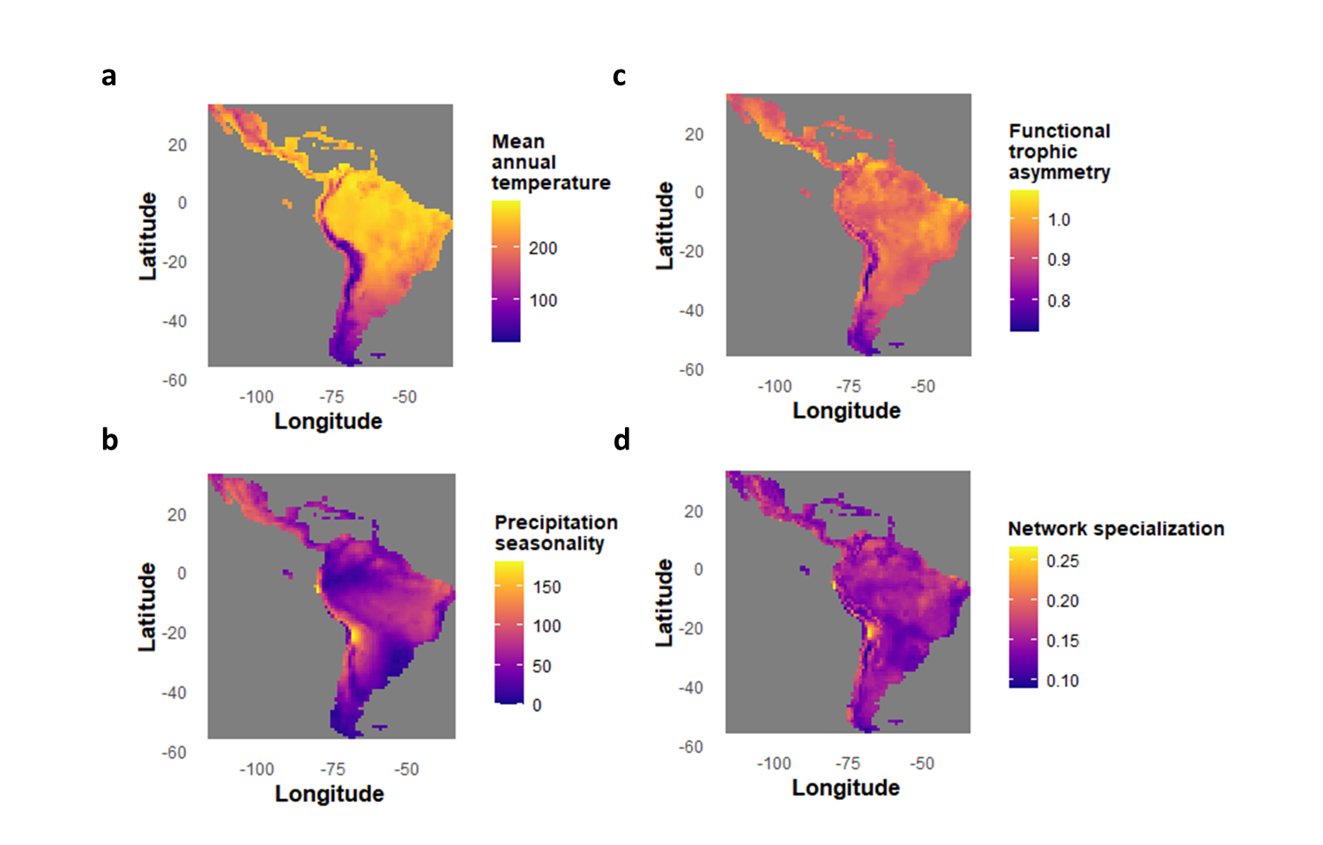
\includegraphics[keepaspectratio]{images/00_Figure06.png}}

}

\caption{\label{fig-06}Spatial distribution of climate, functional
trophic asymmetry, and network specialization for palm-mammal frugivore
seed dispersal networks across the Neotropics. Panels (a) and (a) show
the geographical variation in mean annual temperature and precipitation
seasonality, respectively, with warmer colors indicating higher values.
Panels (c) and (d) depict the spatial patterns of functional trophic
asymmetry (FTA) and network specialization (H2'), where higher values
are also represented by warmer colors. FTA (Panel c) reflects variation
in functional trophic asymmetry across regions, with higher values
concentrated in areas of higher temperature and seasonality. Network
specialization (Panel d) indicates the degree of exclusive interactions
within ecological networks. Color scales for each map are shown in
adjacent legends.}

\end{figure}%

Interaction strength, representing the intensity of the effect that one
species has on another within an ecological network, varies
significantly across palms and mammal frugivore guilds. Moreover,
variation in the strength of interaction between palm-frugivore guilds
mediates the response of FTA to precipitation seasonality. Specifically,
strongly interacting guilds show a more significant and positive
relationship between FTA and precipitation seasonality. In other words,
palm species among guilds with more specialized seed dispersal are more
common while palm species among guilds with a generalist seed dispersal
strategy become rarer towards regions where rainfall is seasonal (Figure
5b, 5d). As precipitation becomes more seasonal, palm functional
richness shifts towards large-fruited species and mammal frugivore
generalists become scarcer. Our results align with findings such as from
bat-plant mutualistic pollination networks, where interacting species
exhibit lower niche overlap in highly seasonal environments, and for
avian-frugivory networks where weaker trait matching is found towards
the tropics (Huang et al., 2025; Schleuning et al., 2012), but also
contrast with others that report stronger trait-matching and interaction
strength towards the tropics in plant-hummingbird pollination networks
(Sonne et al., 2020) and avian-palm frugivory (McFadden et al., 2022).

The concept of functional trophic asymmetry (FTA) offers a valuable
framework to examine how multitrophic ecological communities respond to
shifting environmental conditions. Our results suggest that as global
climate change accelerates, rising temperatures and altered
precipitation regimes are likely to increase FTA multitrophic
palm-frugivore communities and increase specialization in palm seed
dispersal networks. A likely consequence is also the loss of ecosystem
function, namely plant functional connectivity ---the dispersal of plant
propagules between habitat patches---, which has been shown to decrease
with increased specialization and reduced plant functional diversity
(Landim et al., 2025). The same could be true of other ecosystem
functions in other types of mutualistic networks, but it remains to be
explored (Acosta-Rojas et al., 2023; Landim et al., 2025; Nowak et al.,
2025; Rabeau et al., 2025). In addition to climate change, habitat
fragmentation and human-induced landscape modifications can
independently alter resource and consumer functional diversity, thereby
affecting FTA (Béllo Carvalho et al., 2023; Guevara et al., n.d.).
Although differences in the extent of landscape fragmentation were not
directly investigated in this study, previous research shows that
deforestation has a greater impact on the diversity and redundancy of
functional roles in plants than in their hummingbird pollinators,
suggesting a decline in plant functional roles as forests are lost. Such
results reinforce the role of FTA as a key indicator in predicting
shifts in ecosystem function (Bello et al., 2023; Brodie et al., 2021;
Montoya \& Raffaelli, 2010)as species distributions shift in response to
climate change (Aizen et al., 2012; Bartley et al., 2019; Hurtado et
al., 2024; Valiente-Banuet et al., 2015). Adding additional information
such as geographical variation in population density, land-use change,
or spatial movement data (e.g., GPS tracking of frugivores) would
improve realism and generalization of our models (Beumer et al., 2025;
Borah et al., 2022; Cousens et al., 2010). Future work can integrate
these elements into our data pipelines once the relevant data becomes
available.

\subsection{Supplementary material:}\label{supplementary-material}

\subsubsection{Supplementary figures}\label{supplementary-figures}

\subsubsection{Figure S1}

\begin{figure}[H]

{\centering \pandocbounded{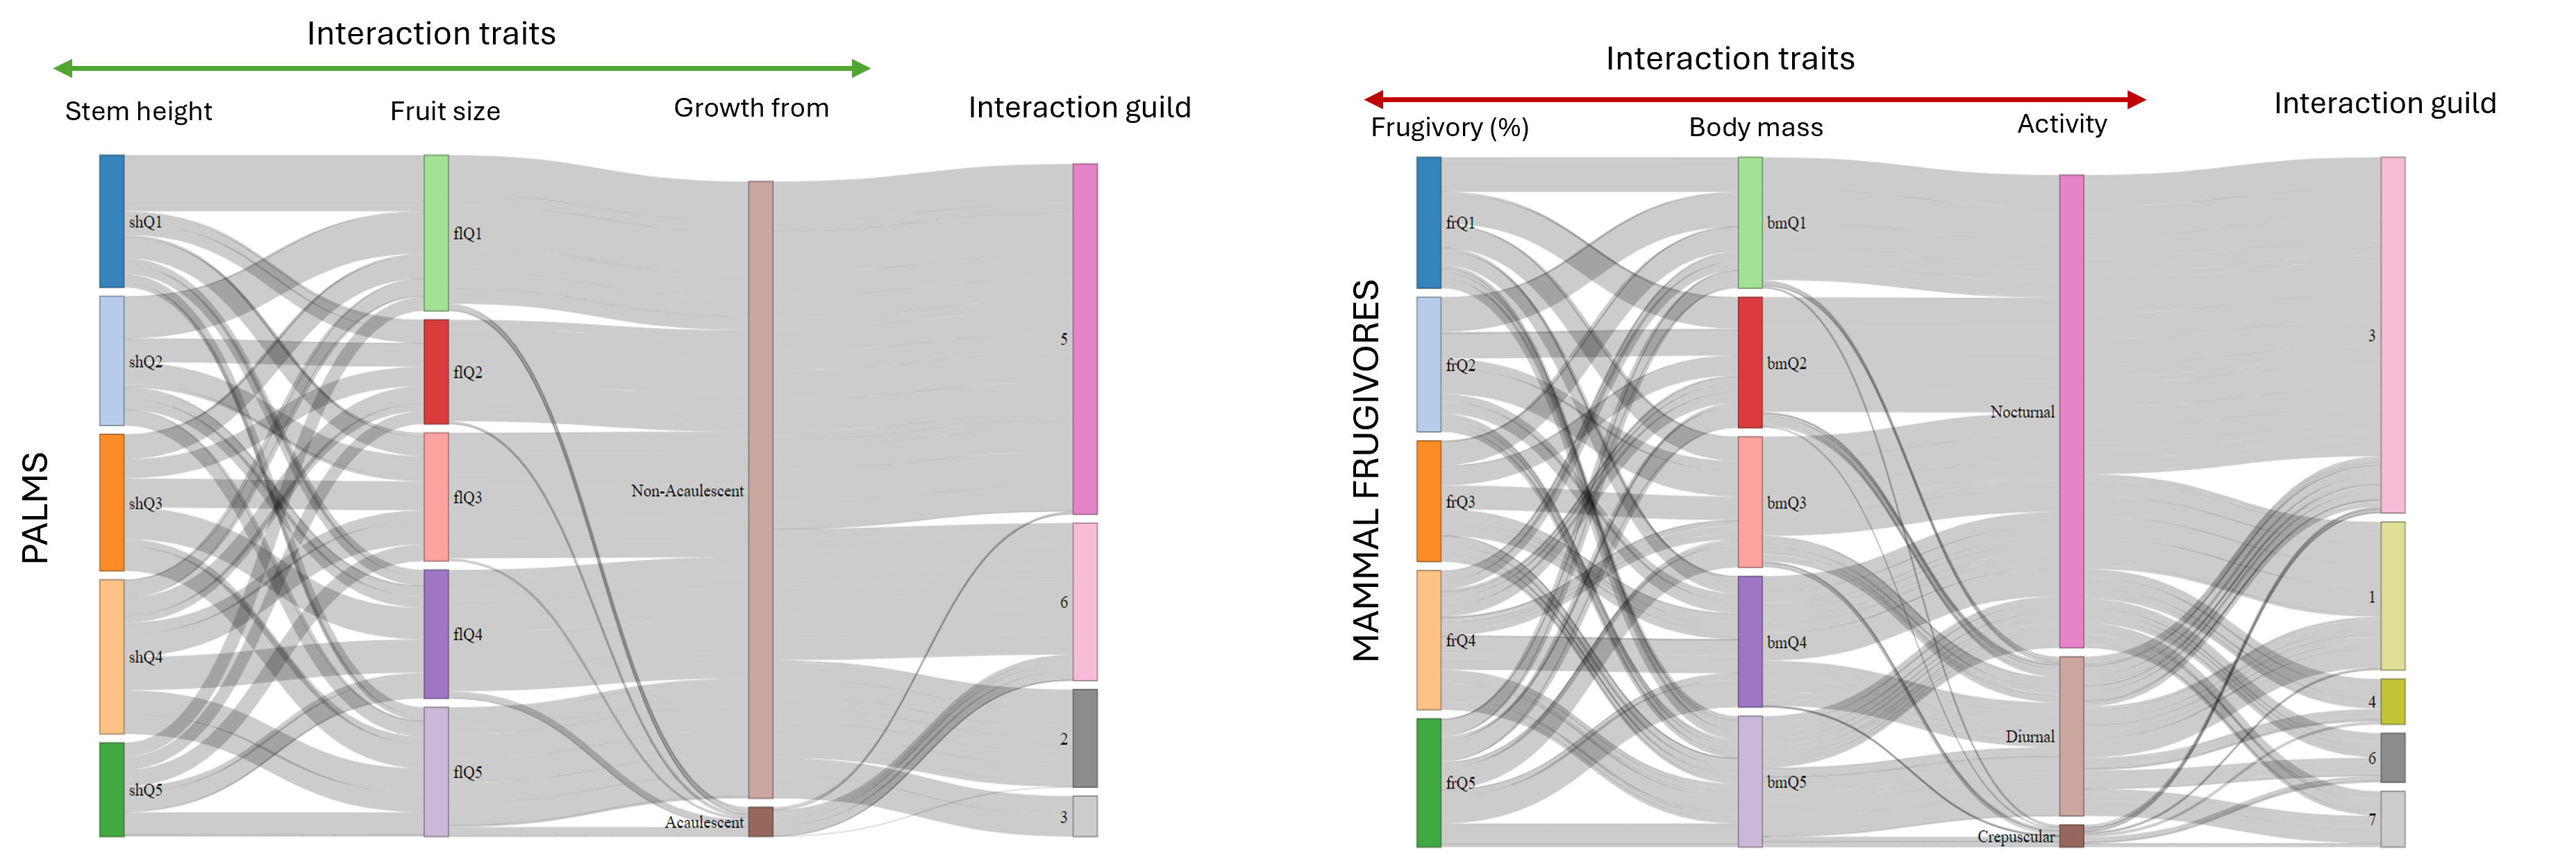
\includegraphics[keepaspectratio]{images/Sup_Mat/00_FigureS1.png}}

}

\caption{Sankey diagrams illustrating the differences in trait
associations to an interaction guild across trophic levels. Top panel -
palms: Relationships between stem height and fruit size, followed by a
growth form classification (Aculescent vs.~Non-Aculescent). Bottom
panel-mammal frugivores: Relationships between percentage frugivory in
diet and body size categorized into different activity periods
(Nocturnal, Diurnal, and Crepuscular). Stem height, Fruit size,
Frugivory (\%) and Body mass are continuous traits that are grouped into
quintiles for visualization purposes. Interaction guilds are defined for
both groups with Stochastic Block Modelling of the palm-mammal frugivore
interaction aggregated metaweb for the Neotropics. Trait associations to
interaction guilds were discovered through multinomial classification
modelling using a neural network backend.}

\end{figure}%

\subsubsection{Figure S2}

\begin{figure}[H]

{\centering \pandocbounded{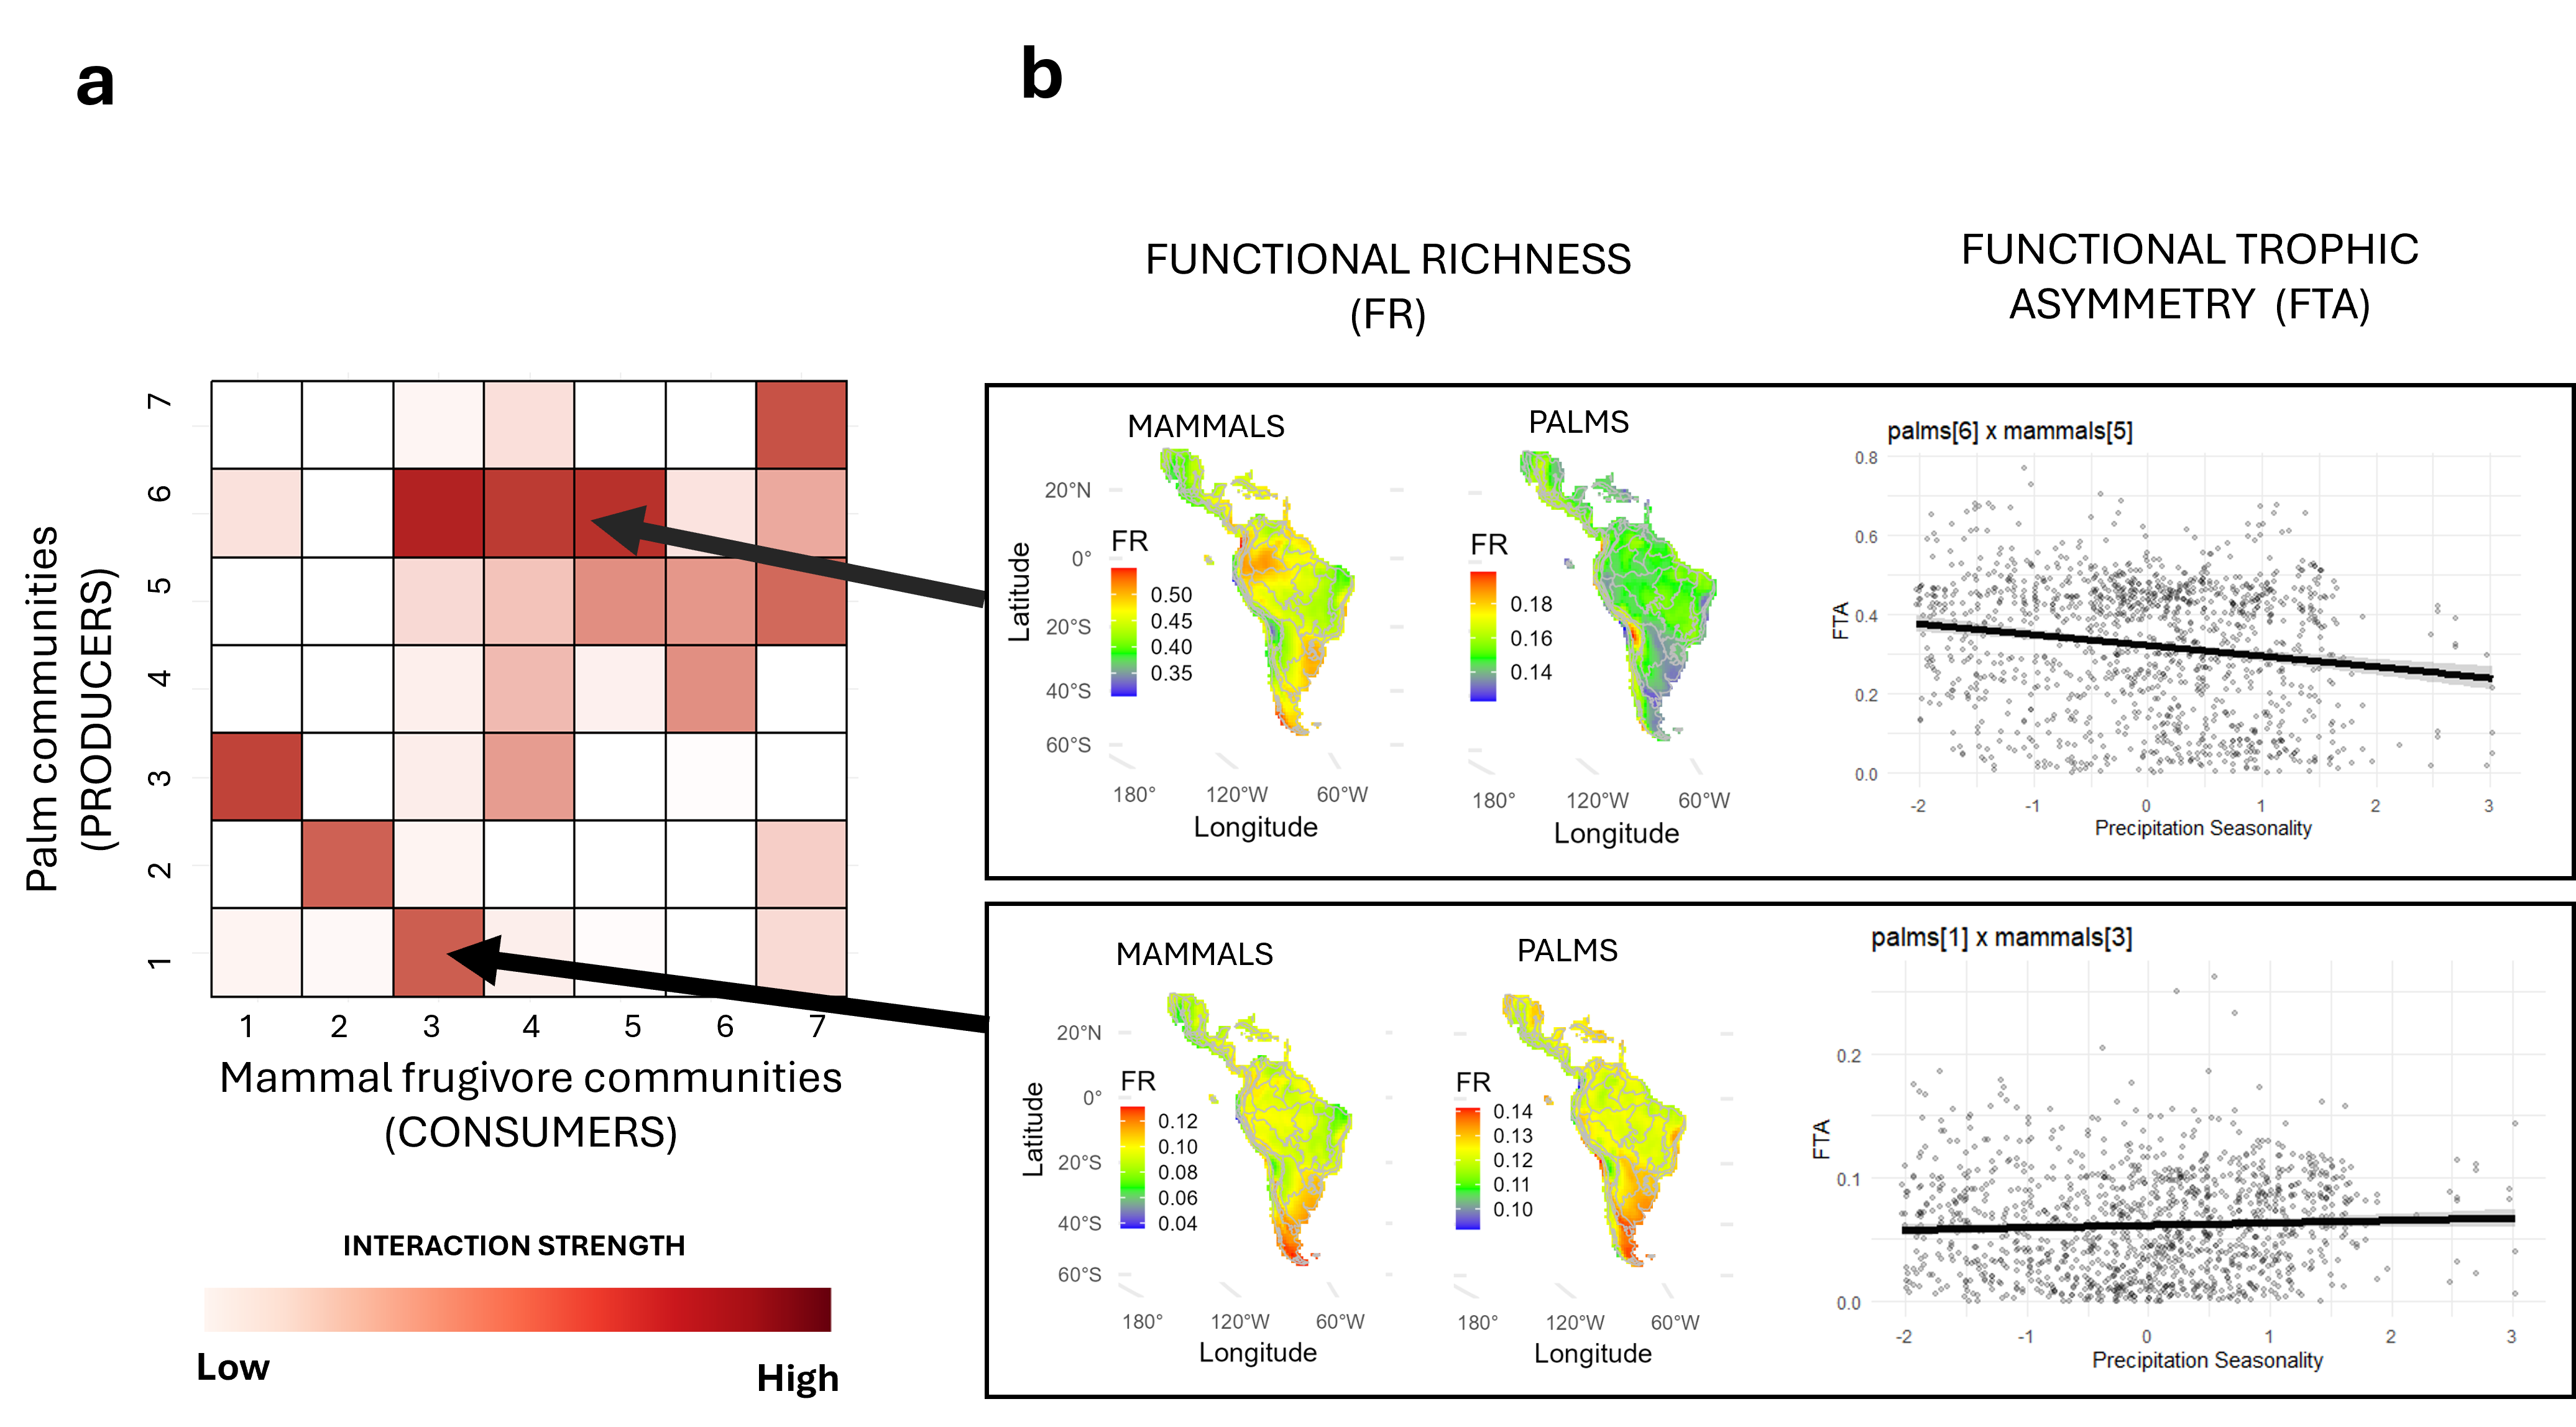
\includegraphics[keepaspectratio]{images/Sup_Mat/00_FigureS2.png}}

}

\caption{Computing functional asymmetry across distinct interaction
guilds. The figure (a) refers to the theta matrix summarizing distinct
interaction guilds betrween producers and consumers with shades of red
representing the strenght of interactions between species within and
between guilds. The figure (b) illustrates two cases of FTA. The panel
above illustrates a guild where FTA changes along the environmental
gradient (precipitation seasonality, panel below illustrates a case
where FTA remains relatively constant )}

\end{figure}%

\subsubsection{Figure S3}

\begin{figure}[H]

{\centering \pandocbounded{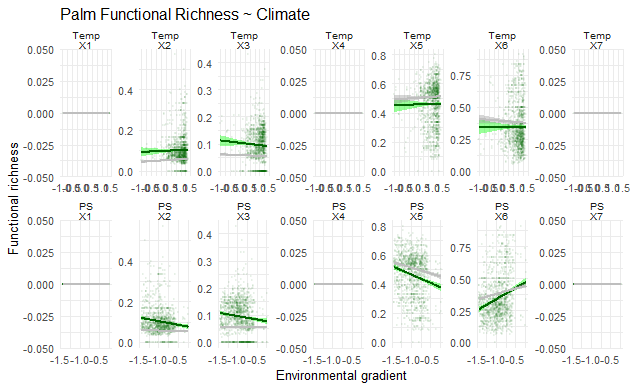
\includegraphics[keepaspectratio]{images/Sup_Mat/00_FigureS4.png}}

}

\caption{Changes in the functional richness of palms along gradients of
temperature and precipitation seasonality. Each pane represents the
trend of the communities of mammals in a single interaction guild. Green
lines represent observed trends, gray lines represent expected trends
from a null model.}

\end{figure}%

\subsubsection{Figure S4}

\begin{figure}[H]

{\centering \pandocbounded{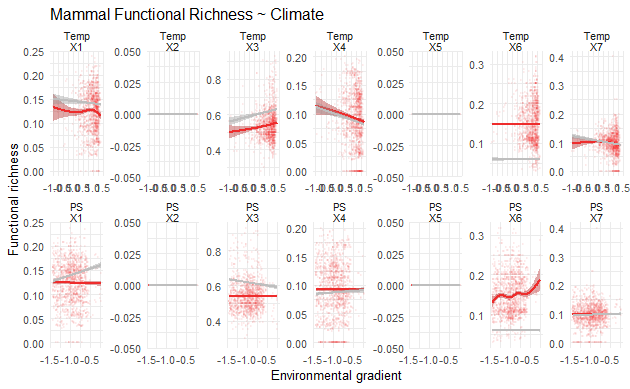
\includegraphics[keepaspectratio]{images/Sup_Mat/00_FigureS3.png}}

}

\caption{Changes in the functional richness of mammals along gradients
of temperature and precipitation seasonality. Each pane represents the
trend of the communities of mammals in a single interaction guild. Red
lines represent observed trends, gray lines represent expected trends
from a null model}

\end{figure}%

\subsubsection{Figure S5}

\begin{figure}[H]

{\centering \pandocbounded{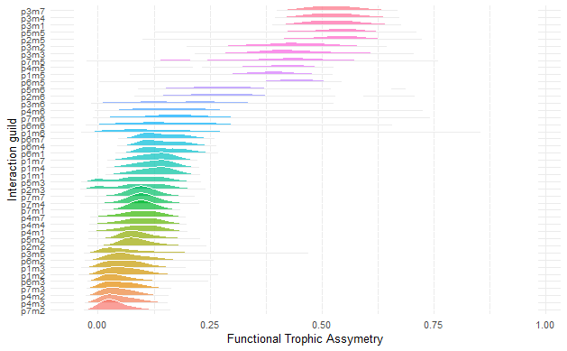
\includegraphics[keepaspectratio]{images/Sup_Mat/00_Figure_S5.png}}

}

\caption{Functional trophic asymmetry across interaction guilds.
Histograms show the distribution of FTA across each combination of palm
(p) and mammal (m) guilds across the Neotropics.}

\end{figure}%

\subsubsection{Figure S6}

\begin{figure}[H]

{\centering \pandocbounded{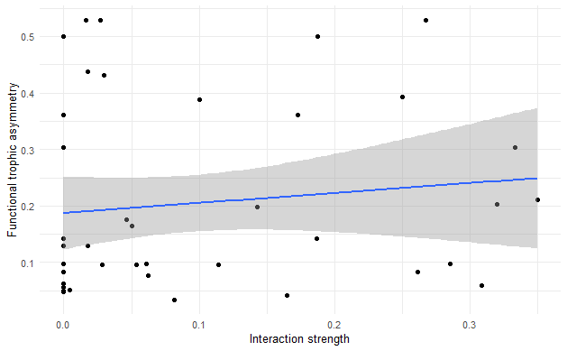
\includegraphics[keepaspectratio]{images/Sup_Mat/00_Figure_S6.png}}

}

\caption{The relationship between Functional Trophic Asymmetry and
Interaction Strength. The y-axis represents the median FTA of an
interaction guild. The x-axis represents the interaction strength,
measured by their interaction probability between guilds modelled by a
stochastic block model (SBM)}

\end{figure}%

\subsubsection{Figure S7}

\begin{figure}[H]

{\centering \pandocbounded{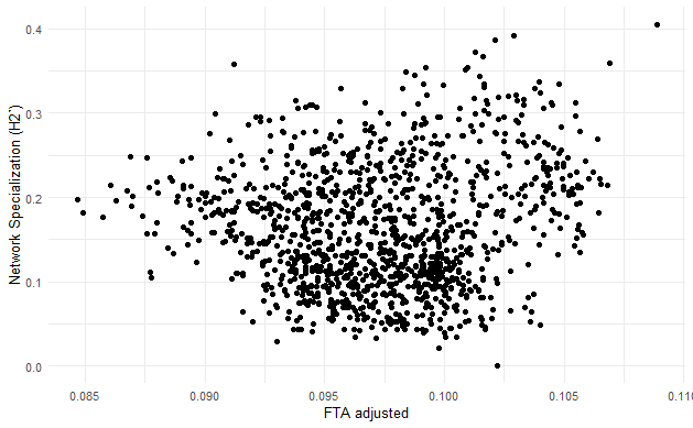
\includegraphics[keepaspectratio]{images/Sup_Mat/00_FigureS9.png}}

}

\caption{The relationship between Network specialization and FTA
(adjusted for interaction strength)}

\end{figure}%

\subsubsection{Figure S8}

\begin{figure}[H]

{\centering \pandocbounded{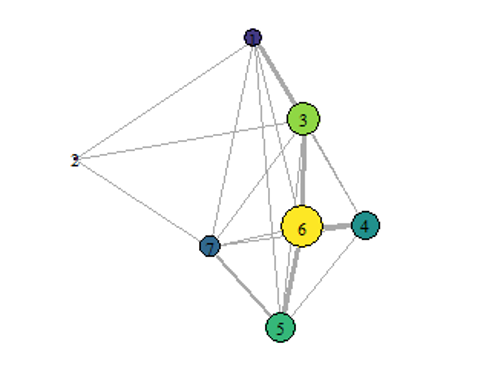
\includegraphics[keepaspectratio]{images/Sup_Mat/00_FigureS10.png}}

}

\caption{The relative influence of distinct nteraction guilds on
mantaining the strupalm-seed dispersal networks in the structure
Neotropics. Nodes represent a consumer/producer guild and links
represents interactions among them. The size of nodes highlights the
node-centrality, a measure of connectivity and influence over other
nodes in the network.}

\end{figure}%

\subsubsection{Supplementary tables}\label{supplementary-tables}

\begin{tcolorbox}[enhanced jigsaw, colframe=quarto-callout-color-frame, opacityback=0, bottomrule=.15mm, left=2mm, toprule=.15mm, arc=.35mm, rightrule=.15mm, colback=white, breakable, leftrule=.75mm]

\vspace{-3mm}\textbf{Table S1}\vspace{3mm}

Summary of parametric and smooth term coefficients for models predicting
ecological responses in the Functional Richness of interaction relevant
traits of Palms. The parametric coefficients include estimates, standard
errors, t-values, and p-values for each predictor (Intercept, Mean
annual temperature (Temp), Total annual precipitation (Prec),
Temperature seasonality (TS), and Precipitation seasonality (PS) ).
Smooth terms are shown for each predictor in combination with ecological
guilds (Guild\_X1 through Guild\_X7), providing the effective degrees of
freedom (edf), reference degrees of freedom (Ref.df), F-statistics, and
p-values for each interaction. Significant p-values are highlighted,
indicating where predictor-guild interactions have a statistically
significant effect on the response variable.

\begin{longtable}[]{@{}
  >{\centering\arraybackslash}p{(\linewidth - 6\tabcolsep) * \real{0.2500}}
  >{\centering\arraybackslash}p{(\linewidth - 6\tabcolsep) * \real{0.2500}}
  >{\centering\arraybackslash}p{(\linewidth - 6\tabcolsep) * \real{0.2500}}
  >{\centering\arraybackslash}p{(\linewidth - 6\tabcolsep) * \real{0.2500}}@{}}
\toprule\noalign{}
\endhead
\bottomrule\noalign{}
\endlastfoot
~ &
\multicolumn{3}{>{\centering\arraybackslash}p{(\linewidth - 6\tabcolsep) * \real{0.7500} + 4\tabcolsep}@{}}{%
Dependent variable} \\
Predictors & Estimates & CI & p \\
(Intercept) & 0.01 & -0.01~--~0.03 & 0.335 \\
Temp & 0.00 & 0.00~--~0.00 & \textbf{0.003} \\
Prec & 0.00 & -0.00~--~0.00 & 0.233 \\
TS & -0.00 & -0.00~--~0.00 & 0.789 \\
PS & 0.00 & -0.00~--~0.00 & 0.499 \\
\begin{minipage}[t]{\linewidth}\raggedright
Smooth term (Temp) × SBM\\
GX1\strut
\end{minipage} & & & 0.073 \\
\begin{minipage}[t]{\linewidth}\raggedright
Smooth term (Temp) × SBM\\
GX2\strut
\end{minipage} & & & 0.129 \\
\begin{minipage}[t]{\linewidth}\raggedright
Smooth term (Temp) × SBM\\
GX3\strut
\end{minipage} & & & \textbf{0.014} \\
\begin{minipage}[t]{\linewidth}\raggedright
Smooth term (Temp) × SBM\\
GX4\strut
\end{minipage} & & & 0.073 \\
\begin{minipage}[t]{\linewidth}\raggedright
Smooth term (Temp) × SBM\\
GX5\strut
\end{minipage} & & & 0.067 \\
\begin{minipage}[t]{\linewidth}\raggedright
Smooth term (Temp) × SBM\\
GX6\strut
\end{minipage} & & & 0.207 \\
\begin{minipage}[t]{\linewidth}\raggedright
Smooth term (Temp) × SBM\\
GX7\strut
\end{minipage} & & & 0.073 \\
\begin{minipage}[t]{\linewidth}\raggedright
Smooth term (Prec) × SBM\\
GX1\strut
\end{minipage} & & & 0.331 \\
\begin{minipage}[t]{\linewidth}\raggedright
Smooth term (Prec) × SBM\\
GX2\strut
\end{minipage} & & & 0.292 \\
\begin{minipage}[t]{\linewidth}\raggedright
Smooth term (Prec) × SBM\\
GX3\strut
\end{minipage} & & & 0.392 \\
\begin{minipage}[t]{\linewidth}\raggedright
Smooth term (Prec) × SBM\\
GX4\strut
\end{minipage} & & & 0.331 \\
\begin{minipage}[t]{\linewidth}\raggedright
Smooth term (Prec) × SBM\\
GX5\strut
\end{minipage} & & & 0.637 \\
\begin{minipage}[t]{\linewidth}\raggedright
Smooth term (Prec) × SBM\\
GX6\strut
\end{minipage} & & & \textbf{0.007} \\
\begin{minipage}[t]{\linewidth}\raggedright
Smooth term (Prec) × SBM\\
GX7\strut
\end{minipage} & & & 0.331 \\
\begin{minipage}[t]{\linewidth}\raggedright
Smooth term (TS) × SBM\\
GX1\strut
\end{minipage} & & & 0.864 \\
\begin{minipage}[t]{\linewidth}\raggedright
Smooth term (TS) × SBM\\
GX2\strut
\end{minipage} & & & 0.863 \\
\begin{minipage}[t]{\linewidth}\raggedright
Smooth term (TS) × SBM\\
GX3\strut
\end{minipage} & & & 0.868 \\
\begin{minipage}[t]{\linewidth}\raggedright
Smooth term (TS) × SBM\\
GX4\strut
\end{minipage} & & & 0.864 \\
\begin{minipage}[t]{\linewidth}\raggedright
Smooth term (TS) × SBM\\
GX5\strut
\end{minipage} & & & 0.890 \\
\begin{minipage}[t]{\linewidth}\raggedright
Smooth term (TS) × SBM\\
GX6\strut
\end{minipage} & & & 0.352 \\
\begin{minipage}[t]{\linewidth}\raggedright
Smooth term (TS) × SBM\\
GX7\strut
\end{minipage} & & & 0.864 \\
\begin{minipage}[t]{\linewidth}\raggedright
Smooth term (PS) × SBM\\
GX1\strut
\end{minipage} & & & 0.705 \\
\begin{minipage}[t]{\linewidth}\raggedright
Smooth term (PS) × SBM\\
GX2\strut
\end{minipage} & & & 0.199 \\
\begin{minipage}[t]{\linewidth}\raggedright
Smooth term (PS) × SBM\\
GX3\strut
\end{minipage} & & & 0.239 \\
\begin{minipage}[t]{\linewidth}\raggedright
Smooth term (PS) × SBM\\
GX4\strut
\end{minipage} & & & 0.705 \\
\begin{minipage}[t]{\linewidth}\raggedright
Smooth term (PS) × SBM\\
GX5\strut
\end{minipage} & & & \textbf{0.007} \\
\begin{minipage}[t]{\linewidth}\raggedright
Smooth term (PS) × SBM\\
GX6\strut
\end{minipage} & & & \textbf{0.001} \\
\begin{minipage}[t]{\linewidth}\raggedright
Smooth term (PS) × SBM\\
GX7\strut
\end{minipage} & & & 0.705 \\
Observations &
\multicolumn{3}{>{\raggedright\arraybackslash}p{(\linewidth - 6\tabcolsep) * \real{0.7500} + 4\tabcolsep}@{}}{%
9009} \\
R\textsuperscript{2} &
\multicolumn{3}{>{\raggedright\arraybackslash}p{(\linewidth - 6\tabcolsep) * \real{0.7500} + 4\tabcolsep}@{}}{%
0.012} \\
\end{longtable}

\textsubscript{Source:
\href{https://lessardlab.github.io/fta_ec_networks/index-preview.html}{Article
Notebook}}

\end{tcolorbox}

\begin{tcolorbox}[enhanced jigsaw, colframe=quarto-callout-color-frame, opacityback=0, bottomrule=.15mm, left=2mm, toprule=.15mm, arc=.35mm, rightrule=.15mm, colback=white, breakable, leftrule=.75mm]

\vspace{-3mm}\textbf{Table S2}\vspace{3mm}

Summary of parametric and smooth term coefficients for models predicting
ecological responses in the Functional Richness of interaction relevant
traits of frugivore Mammals. The parametric coefficients include
estimates, standard errors, t-values, and p-values for each predictor
(Intercept, Mean annual temperature (Temp), Total annual precipitation
(Prec), Temperature seasonality (TS), and Precipitation seasonality (PS)
). Smooth terms are shown for each predictor in combination with
ecological guilds (Guild\_X1 through Guild\_X7), providing the effective
degrees of freedom (edf), reference degrees of freedom (Ref.df),
F-statistics, and p-values for each interaction. Significant p-values
are highlighted, indicating where predictor-guild interactions have a
statistically significant effect on the response variable.

\begin{longtable}[]{@{}
  >{\centering\arraybackslash}p{(\linewidth - 6\tabcolsep) * \real{0.2500}}
  >{\centering\arraybackslash}p{(\linewidth - 6\tabcolsep) * \real{0.2500}}
  >{\centering\arraybackslash}p{(\linewidth - 6\tabcolsep) * \real{0.2500}}
  >{\centering\arraybackslash}p{(\linewidth - 6\tabcolsep) * \real{0.2500}}@{}}
\toprule\noalign{}
\endhead
\bottomrule\noalign{}
\endlastfoot
~ &
\multicolumn{3}{>{\centering\arraybackslash}p{(\linewidth - 6\tabcolsep) * \real{0.7500} + 4\tabcolsep}@{}}{%
Dependent variable} \\
Predictors & Estimates & CI & p \\
(Intercept) & 0.01 & -0.01~--~0.03 & 0.335 \\
Temp & 0.00 & 0.00~--~0.00 & \textbf{0.003} \\
Prec & 0.00 & -0.00~--~0.00 & 0.233 \\
TS & -0.00 & -0.00~--~0.00 & 0.789 \\
PS & 0.00 & -0.00~--~0.00 & 0.499 \\
\begin{minipage}[t]{\linewidth}\raggedright
Smooth term (Temp) × SBM\\
GX1\strut
\end{minipage} & & & 0.073 \\
\begin{minipage}[t]{\linewidth}\raggedright
Smooth term (Temp) × SBM\\
GX2\strut
\end{minipage} & & & 0.129 \\
\begin{minipage}[t]{\linewidth}\raggedright
Smooth term (Temp) × SBM\\
GX3\strut
\end{minipage} & & & \textbf{0.014} \\
\begin{minipage}[t]{\linewidth}\raggedright
Smooth term (Temp) × SBM\\
GX4\strut
\end{minipage} & & & 0.073 \\
\begin{minipage}[t]{\linewidth}\raggedright
Smooth term (Temp) × SBM\\
GX5\strut
\end{minipage} & & & 0.067 \\
\begin{minipage}[t]{\linewidth}\raggedright
Smooth term (Temp) × SBM\\
GX6\strut
\end{minipage} & & & 0.207 \\
\begin{minipage}[t]{\linewidth}\raggedright
Smooth term (Temp) × SBM\\
GX7\strut
\end{minipage} & & & 0.073 \\
\begin{minipage}[t]{\linewidth}\raggedright
Smooth term (Prec) × SBM\\
GX1\strut
\end{minipage} & & & 0.331 \\
\begin{minipage}[t]{\linewidth}\raggedright
Smooth term (Prec) × SBM\\
GX2\strut
\end{minipage} & & & 0.292 \\
\begin{minipage}[t]{\linewidth}\raggedright
Smooth term (Prec) × SBM\\
GX3\strut
\end{minipage} & & & 0.392 \\
\begin{minipage}[t]{\linewidth}\raggedright
Smooth term (Prec) × SBM\\
GX4\strut
\end{minipage} & & & 0.331 \\
\begin{minipage}[t]{\linewidth}\raggedright
Smooth term (Prec) × SBM\\
GX5\strut
\end{minipage} & & & 0.637 \\
\begin{minipage}[t]{\linewidth}\raggedright
Smooth term (Prec) × SBM\\
GX6\strut
\end{minipage} & & & \textbf{0.007} \\
\begin{minipage}[t]{\linewidth}\raggedright
Smooth term (Prec) × SBM\\
GX7\strut
\end{minipage} & & & 0.331 \\
\begin{minipage}[t]{\linewidth}\raggedright
Smooth term (TS) × SBM\\
GX1\strut
\end{minipage} & & & 0.864 \\
\begin{minipage}[t]{\linewidth}\raggedright
Smooth term (TS) × SBM\\
GX2\strut
\end{minipage} & & & 0.863 \\
\begin{minipage}[t]{\linewidth}\raggedright
Smooth term (TS) × SBM\\
GX3\strut
\end{minipage} & & & 0.868 \\
\begin{minipage}[t]{\linewidth}\raggedright
Smooth term (TS) × SBM\\
GX4\strut
\end{minipage} & & & 0.864 \\
\begin{minipage}[t]{\linewidth}\raggedright
Smooth term (TS) × SBM\\
GX5\strut
\end{minipage} & & & 0.890 \\
\begin{minipage}[t]{\linewidth}\raggedright
Smooth term (TS) × SBM\\
GX6\strut
\end{minipage} & & & 0.352 \\
\begin{minipage}[t]{\linewidth}\raggedright
Smooth term (TS) × SBM\\
GX7\strut
\end{minipage} & & & 0.864 \\
\begin{minipage}[t]{\linewidth}\raggedright
Smooth term (PS) × SBM\\
GX1\strut
\end{minipage} & & & 0.705 \\
\begin{minipage}[t]{\linewidth}\raggedright
Smooth term (PS) × SBM\\
GX2\strut
\end{minipage} & & & 0.199 \\
\begin{minipage}[t]{\linewidth}\raggedright
Smooth term (PS) × SBM\\
GX3\strut
\end{minipage} & & & 0.239 \\
\begin{minipage}[t]{\linewidth}\raggedright
Smooth term (PS) × SBM\\
GX4\strut
\end{minipage} & & & 0.705 \\
\begin{minipage}[t]{\linewidth}\raggedright
Smooth term (PS) × SBM\\
GX5\strut
\end{minipage} & & & \textbf{0.007} \\
\begin{minipage}[t]{\linewidth}\raggedright
Smooth term (PS) × SBM\\
GX6\strut
\end{minipage} & & & \textbf{0.001} \\
\begin{minipage}[t]{\linewidth}\raggedright
Smooth term (PS) × SBM\\
GX7\strut
\end{minipage} & & & 0.705 \\
Observations &
\multicolumn{3}{>{\raggedright\arraybackslash}p{(\linewidth - 6\tabcolsep) * \real{0.7500} + 4\tabcolsep}@{}}{%
9009} \\
R\textsuperscript{2} &
\multicolumn{3}{>{\raggedright\arraybackslash}p{(\linewidth - 6\tabcolsep) * \real{0.7500} + 4\tabcolsep}@{}}{%
0.012} \\
\end{longtable}

\textsubscript{Source:
\href{https://lessardlab.github.io/fta_ec_networks/index-preview.html}{Article
Notebook}}

\end{tcolorbox}

\subsubsection*{Supplementary text}\label{supplementary-text}
\addcontentsline{toc}{subsubsection}{Supplementary text}

\phantomsection\label{refs}
\begin{CSLReferences}{1}{0}
\bibitem[\citeproctext]{ref-acevedo2020structure}
Acevedo-Quintero, J. F., Zamora-Abrego, J. G., \& Garcı́a, D. (2020).
From structure to function in mutualistic interaction networks:
Topologically important frugivores have greater potential as seed
dispersers. \emph{Journal of Animal Ecology}, \emph{89}(9), 2181--2191.

\bibitem[\citeproctext]{ref-ackerly2003community}
Ackerly, D. D. (2003). Community assembly, niche conservatism, and
adaptive evolution in changing environments. \emph{International Journal
of Plant Sciences}, \emph{164}(S3), S165--S184.

\bibitem[\citeproctext]{ref-acosta2023abiotic}
Acosta-Rojas, D. C., Barczyk, M. K., Espinosa, C. I., Farwig, N.,
Homeier, J., Tiede, Y., et al. (2023). Abiotic factors similarly shape
the distribution of fruit, seed and leaf traits in tropical
fleshy-fruited tree communities. \emph{Acta Oecologica}, \emph{121},
103953.

\bibitem[\citeproctext]{ref-aizen2012specialization}
Aizen, M. A., Sabatino, M., \& Tylianakis, J. M. (2012). Specialization
and rarity predict nonrandom loss of interactions from mutualist
networks. \emph{Science}, \emph{335}(6075), 1486--1489.

\bibitem[\citeproctext]{ref-albrecht2018plant}
Albrecht, J., Classen, A., Vollstädt, M. G., Mayr, A., Mollel, N. P.,
Schellenberger Costa, D., et al. (2018). Plant and animal functional
diversity drive mutualistic network assembly across an elevational
gradient. \emph{Nature Communications}, \emph{9}(1), 3177.

\bibitem[\citeproctext]{ref-allen2006patterns}
Allen, C. R., Garmestani, A., Havlicek, T., Marquet, P. A., Peterson,
G., Restrepo, C., et al. (2006). Patterns in body mass distributions:
Sifting among alternative hypotheses. \emph{Ecology Letters},
\emph{9}(5), 630--643.

\bibitem[\citeproctext]{ref-allesina2008general}
Allesina, S., Alonso, D., \& Pascual, M. (2008). A general model for
food web structure. \emph{Science}, \emph{320}(5876), 658--661.

\bibitem[\citeproctext]{ref-arends2001comparative}
Arends, A., \& McNab, B. K. (2001). The comparative energetics of
`caviomorph'rodents. \emph{Comparative Biochemistry and Physiology Part
A: Molecular \& Integrative Physiology}, \emph{130}(1), 105--122.

\bibitem[\citeproctext]{ref-bartley2019food}
Bartley, T. J., McCann, K. S., Bieg, C., Cazelles, K., Granados, M.,
Guzzo, M. M., et al. (2019). Food web rewiring in a changing world.
\emph{Nature Ecology \& Evolution}, \emph{3}(3), 345--354.

\bibitem[\citeproctext]{ref-bello2023analyzing}
Bello, C., Schleuning, M., \& Graham, C. H. (2023). Analyzing trophic
ecosystem functions with the interaction functional space. \emph{Trends
in Ecology \& Evolution}, \emph{38}(5), 424--434.

\bibitem[\citeproctext]{ref-bello2023frugivory}
Béllo Carvalho, R., Malhi, Y., \& Oliveras Menor, I. (2023). Frugivory
and seed dispersal in the cerrado: Network structure and defaunation
effects. \emph{Biotropica}, \emph{55}(4), 849--865.

\bibitem[\citeproctext]{ref-beumer2025movetraits}
Beumer, L. T., Hertel, A. G., Royaute, R., Tucker, M. A., Albrecht, J.,
Beltran, R., et al. (2025). MoveTraits-a database for integrating animal
behaviour into trait-based ecology. \emph{bioRxiv}, 2025--03.

\bibitem[\citeproctext]{ref-bjorholm2005environmental}
Bjorholm, S., Svenning, J.-C., Skov, F., \& Balslev, H. (2005).
Environmental and spatial controls of palm (arecaceae) species richness
across the americas. \emph{Global Ecology and Biogeography},
\emph{14}(5), 423--429.

\bibitem[\citeproctext]{ref-bluthgen2011functional}
Blüthgen, N., \& Klein, A.-M. (2011). Functional complementarity and
specialisation: The role of biodiversity in plant--pollinator
interactions. \emph{Basic and Applied Ecology}, \emph{12}(4), 282--291.

\bibitem[\citeproctext]{ref-bluthgen2006measuring}
Blüthgen, N., Menzel, F., \& Blüthgen, N. (2006). Measuring
specialization in species interaction networks. \emph{BMC Ecology},
\emph{6}, 1--12.

\bibitem[\citeproctext]{ref-bluthgen2007specialization}
Blüthgen, N., Menzel, F., Hovestadt, T., Fiala, B., \& Blüthgen, N.
(2007). Specialization, constraints, and conflicting interests in
mutualistic networks. \emph{Current Biology}, \emph{17}(4), 341--346.

\bibitem[\citeproctext]{ref-bogoni2020extent}
Bogoni, J. A., Peres, C. A., \& Ferraz, K. M. (2020). Extent, intensity
and drivers of mammal defaunation: A continental-scale analysis across
the neotropics. \emph{Scientific Reports}, \emph{10}(1), 14750.

\bibitem[\citeproctext]{ref-borah2022seasonal}
Borah, D. K., Solanki, G., \& Bhattacharjee, P. C. (2022). Seasonal
variations in home range size of capped langur (trachypithecus pileatus)
in a degraded habitat in assam, india. \emph{Ecological Questions},
\emph{33}(3), 59--66.

\bibitem[\citeproctext]{ref-brodie2021decline}
Brodie, J. F., Williams, S., \& Garner, B. (2021). The decline of mammal
functional and evolutionary diversity worldwide. \emph{Proceedings of
the National Academy of Sciences}, \emph{118}(3), e1921849118.

\bibitem[\citeproctext]{ref-cousens2010towards}
Cousens, R. D., Hill, J., French, K., \& Bishop, I. D. (2010). Towards
better prediction of seed dispersal by animals. \emph{Functional
Ecology}, \emph{24}(6), 1163--1170.

\bibitem[\citeproctext]{ref-dehling2016morphology}
Dehling, D. M., Jordano, P., Schaefer, H. M., Böhning-Gaese, K., \&
Schleuning, M. (2016). Morphology predicts species' functional roles and
their degree of specialization in plant--frugivore interactions.
\emph{Proceedings of the Royal Society B: Biological Sciences},
\emph{283}(1823), 20152444.

\bibitem[\citeproctext]{ref-dehling2021specialists}
Dehling, D. M., Bender, I. M., Blendinger, P. G., Böhning-Gaese, K.,
Muñoz, M. C., Neuschulz, E. L., et al. (2021). Specialists and
generalists fulfil important and complementary functional roles in
ecological processes. \emph{Functional Ecology}, \emph{35}(8),
1810--1821.

\bibitem[\citeproctext]{ref-dehling2022contribution}
Dehling, D. M., Barreto, E., \& Graham, C. H. (2022). The contribution
of mutualistic interactions to functional and phylogenetic diversity.
\emph{Trends in Ecology \& Evolution}, \emph{37}(9), 768--776.

\bibitem[\citeproctext]{ref-donoso2017defaunation}
Donoso, I., Schleuning, M., Garcı́a, D., \& Fründ, J. (2017). Defaunation
effects on plant recruitment depend on size matching and size trade-offs
in seed-dispersal networks. \emph{Proceedings of the Royal Society B:
Biological Sciences}, \emph{284}(1855), 20162664.

\bibitem[\citeproctext]{ref-donoso2020downsizing}
Donoso, I., Sorensen, M. C., Blendinger, P. G., Kissling, W. D.,
Neuschulz, E. L., Mueller, T., \& Schleuning, M. (2020). Downsizing of
animal communities triggers stronger functional than structural decay in
seed-dispersal networks. \emph{Nature Communications}, \emph{11}(1),
1582.

\bibitem[\citeproctext]{ref-eiserhardt2011geographical}
Eiserhardt, W. L., Svenning, J.-C., Kissling, W. D., \& Balslev, H.
(2011). Geographical ecology of the palms (arecaceae): Determinants of
diversity and distributions across spatial scales. \emph{Annals of
Botany}, \emph{108}(8), 1391--1416.

\bibitem[\citeproctext]{ref-emer2023intraspecific}
Emer, C., \& Memmott, J. (2023). Intraspecific variation of invaded
pollination networks--the role of pollen-transport, pollen-transfer and
different levels of biological organization. \emph{Perspectives in
Ecology and Conservation}, \emph{21}(2), 151--163.

\bibitem[\citeproctext]{ref-emilio2019embolism}
Emilio, T., Lamarque, L. J., Torres-Ruiz, J. M., King, A., Charrier, G.,
Burlett, R., et al. (2019). Embolism resistance in petioles and leaflets
of palms. \emph{Annals of Botany}, \emph{124}(7), 1173--1183.

\bibitem[\citeproctext]{ref-fick2017worldclim}
Fick, S. E., \& Hijmans, R. J. (2017). WorldClim 2: New 1-km spatial
resolution climate surfaces for global land areas. \emph{International
Journal of Climatology}, \emph{37}(12), 4302--4315.

\bibitem[\citeproctext]{ref-garcia2018frugivore}
Garcı́a, D., Donoso, I., \& Rodrı́guez-Pérez, J. (2018). Frugivore
biodiversity and complementarity in interaction networks enhance
landscape-scale seed dispersal function. \emph{Functional Ecology},
\emph{32}(12), 2742--2752.

\bibitem[\citeproctext]{ref-gevrey2003review}
Gevrey, M., Dimopoulos, I., \& Lek, S. (2003). Review and comparison of
methods to study the contribution of variables in artificial neural
network models. \emph{Ecological Modelling}, \emph{160}(3), 249--264.

\bibitem[\citeproctext]{ref-gorczynski2021tropical}
Gorczynski, D., Hsieh, C., Luciano, J. T., Ahumada, J., Espinosa, S.,
Johnson, S., et al. (2021). Tropical mammal functional diversity
increases with productivity but decreases with anthropogenic
disturbance. \emph{Proceedings of the Royal Society B},
\emph{288}(1945), 20202098.

\bibitem[\citeproctext]{ref-guevara4907880land}
Guevara, E., Duchenne, F., Santander, T., \& Graham, C. H. (n.d.). Land
use change affects the contribution of niche-based processes to
plant-pollinator interactions, with possible consequences for network
structure. \emph{Available at SSRN 4907880}.

\bibitem[\citeproctext]{ref-halpern2008functional}
Halpern, B. S., \& Floeter, S. R. (2008). Functional diversity responses
to changing species richness in reef fish communities. \emph{Marine
Ecology Progress Series}, \emph{364}, 147--156.

\bibitem[\citeproctext]{ref-hillerislambers2012rethinking}
HilleRisLambers, J., Adler, P. B., Harpole, W. S., Levine, J. M., \&
Mayfield, M. M. (2012). Rethinking community assembly through the lens
of coexistence theory. \emph{Annual Review of Ecology, Evolution, and
Systematics}, \emph{43}(1), 227--248.

\bibitem[\citeproctext]{ref-hoekstra2001mechanisms}
Hoekstra, F. A., Golovina, E. A., \& Buitink, J. (2001). Mechanisms of
plant desiccation tolerance. \emph{Trends in Plant Science},
\emph{6}(9), 431--438.

\bibitem[\citeproctext]{ref-holt2018environmental}
Holt, B. G., Costa, G. C., Penone, C., Lessard, J.-P., Brooks, T. M.,
Davidson, A. D., et al. (2018). Environmental variation is a major
predictor of global trait turnover in mammals. \emph{Journal of
Biogeography}, \emph{45}(1), 225--237.

\bibitem[\citeproctext]{ref-huang2025weaker}
Huang, X., Dalsgaard, B., \& Chen, S.-C. (2025). Weaker plant-frugivore
trait matching towards the tropics and on islands. \emph{Ecology
Letters}, \emph{28}(1), e70061.

\bibitem[\citeproctext]{ref-hurtado2024generalism}
Hurtado, P., Aragón, G., Vicente, M., Dalsgaard, B., Krasnov, B. R., \&
Calatayud, J. (2024). Generalism in species interactions is more the
consequence than the cause of ecological success. \emph{Nature Ecology
\& Evolution}, \emph{8}(9), 1602--1611.

\bibitem[\citeproctext]{ref-kissling2012towards}
Kissling, W. D., Dormann, C. F., Groeneveld, J., Hickler, T., Kühn, I.,
McInerny, G. J., et al. (2012). Towards novel approaches to modelling
biotic interactions in multispecies assemblages at large spatial
extents. \emph{Journal of Biogeography}, \emph{39}(12), 2163--2178.

\bibitem[\citeproctext]{ref-kissling2019palmtraits}
Kissling, W. D., Balslev, H., Baker, W. J., Dransfield, J., Göldel, B.,
Lim, J. Y., et al. (2019). PalmTraits 1.0, a species-level functional
trait database of palms worldwide. \emph{Scientific Data}, \emph{6}(1),
178.

\bibitem[\citeproctext]{ref-kraft2010functional}
Kraft, N. J., \& Ackerly, D. D. (2010). Functional trait and
phylogenetic tests of community assembly across spatial scales in an
amazonian forest. \emph{Ecological Monographs}, \emph{80}(3), 401--422.

\bibitem[\citeproctext]{ref-kraft2008functional}
Kraft, N. J., Valencia, R., \& Ackerly, D. D. (2008). Functional traits
and niche-based tree community assembly in an amazonian forest.
\emph{Science}, \emph{322}(5901), 580--582.

\bibitem[\citeproctext]{ref-kraft2015community}
Kraft, N. J., Adler, P. B., Godoy, O., James, E. C., Fuller, S., \&
Levine, J. M. (2015). Community assembly, coexistence and the
environmental filtering metaphor. \emph{Functional Ecology},
\emph{29}(5), 592--599.

\bibitem[\citeproctext]{ref-laliberte2010distance}
Laliberté, E., \& Legendre, P. (2010). A distance-based framework for
measuring functional diversity from multiple traits. \emph{Ecology},
\emph{91}(1), 299--305.

\bibitem[\citeproctext]{ref-landim2025functional}
Landim, A. R., Neuschulz, E. L., Donoso, I., Sorensen, M. C., Mueller,
T., \& Schleuning, M. (2025). Functional connectivity of
animal-dispersed plant communities depends on the interacting effects of
network specialization and resource diversity. \emph{Proceedings B},
\emph{292}(2042), 20242995.

\bibitem[\citeproctext]{ref-lavorel2013plant}
Lavorel, S. (2013). Plant functional effects on ecosystem services.
\emph{Journal of Ecology}. Wiley Online Library.

\bibitem[\citeproctext]{ref-losada2024geographic}
Losada, M., Suárez-Couselo, M., \& Sobral, M. (2024). Geographic
distribution of mammal diets. \emph{Web Ecology}, \emph{24}(2), 71--79.

\bibitem[\citeproctext]{ref-marjakangas2022trait}
Marjakangas, E.-L., Muñoz, G., Turney, S., Albrecht, J., Neuschulz, E.
L., Schleuning, M., \& Lessard, J.-P. (2022). Trait-based inference of
ecological network assembly: A conceptual framework and methodological
toolbox. \emph{Ecological Monographs}, \emph{92}(2), e1502.

\bibitem[\citeproctext]{ref-marques2022mutualism}
Marques Dracxler, C., \& Kissling, W. D. (2022). The
mutualism--antagonism continuum in neotropical palm--frugivore
interactions: From interaction outcomes to ecosystem dynamics.
\emph{Biological Reviews}, \emph{97}(2), 527--553.

\bibitem[\citeproctext]{ref-mccain2014body}
McCain, C. M., \& King, S. R. (2014). Body size and activity times
mediate mammalian responses to climate change. \emph{Global Change
Biology}, \emph{20}(6), 1760--1769.

\bibitem[\citeproctext]{ref-mcfadden2022global}
McFadden, I. R., Fritz, S. A., Zimmermann, N. E., Pellissier, L.,
Kissling, W. D., Tobias, J. A., et al. (2022). Global plant-frugivore
trait matching is shaped by climate and biogeographic history.
\emph{Ecology Letters}, \emph{25}(3), 686--696.

\bibitem[\citeproctext]{ref-merritt2010biology}
Merritt, J. F. (2010). \emph{The biology of small mammals}. JHU Press.

\bibitem[\citeproctext]{ref-messeder2021frugivory}
Messeder, J. V. S., Silveira, F. A., Cornelissen, T. G., Fuzessy, L. F.,
\& Guerra, T. J. (2021). Frugivory and seed dispersal in a hyperdiverse
plant clade and its role as a keystone resource for the neotropical
fauna. \emph{Annals of Botany}, \emph{127}(5), 577--595.

\bibitem[\citeproctext]{ref-montoya2010climate}
Montoya, J. M., \& Raffaelli, D. (2010). Climate change, biotic
interactions and ecosystem services. \emph{Philosophical Transactions of
the Royal Society B: Biological Sciences}, \emph{365}(1549), 2013--2018.

\bibitem[\citeproctext]{ref-moretti2009combining}
Moretti, M., \& Legg, C. (2009). Combining plant and animal traits to
assess community functional responses to disturbance. \emph{Ecography},
\emph{32}(2), 299--309.

\bibitem[\citeproctext]{ref-munoz2019synthesis}
Muñoz, G., Trøjelsgaard, K., \& Kissling, W. D. (2019). A synthesis of
animal-mediated seed dispersal of palms reveals distinct biogeographical
differences in species interactions. \emph{Journal of Biogeography},
\emph{46}(2), 466--484.

\bibitem[\citeproctext]{ref-nowak2025impacts}
Nowak, L., Fricke, E. C., Traveset, A., \& Donoso, I. (2025). Impacts of
species introductions on the trait diversity of interacting avian
frugivores and fleshy-fruited plants depend on native trait diversity.
\emph{bioRxiv}, 2025--01.

\bibitem[\citeproctext]{ref-onstein2014diversification}
Onstein, R. E., Carter, R. J., Xing, Y., \& Linder, H. P. (2014).
Diversification rate shifts in the cape floristic region: The right
traits in the right place at the right time. \emph{Perspectives in Plant
Ecology, Evolution and Systematics}, \emph{16}(6), 331--340.

\bibitem[\citeproctext]{ref-onstein2017frugivory}
Onstein, R. E., Baker, W. J., Couvreur, T. L., Faurby, S., Svenning,
J.-C., \& Kissling, W. D. (2017). Frugivory-related traits promote
speciation of tropical palms. \emph{Nature Ecology \& Evolution},
\emph{1}(12), 1903--1911.

\bibitem[\citeproctext]{ref-paine2011functional}
Paine, C. T., Baraloto, C., Chave, J., \& Hérault, B. (2011). Functional
traits of individual trees reveal ecological constraints on community
assembly in tropical rain forests. \emph{Oikos}, \emph{120}(5),
720--727.

\bibitem[\citeproctext]{ref-poisot2023guidelines}
Poisot, T. (2023). Guidelines for the prediction of species interactions
through binary classification. \emph{Methods in Ecology and Evolution},
\emph{14}(5), 1333--1345.

\bibitem[\citeproctext]{ref-rabeau2025projected}
Rabeau, A., Pigot, A., Tobias, J., \& Schleuning, M. (2025). Projected
impacts of climate change on plant-frugivore interactions across the
americas. \emph{bioRxiv}, 2025--03.

\bibitem[\citeproctext]{ref-reichgelt2018relation}
Reichgelt, T., West, C. K., \& Greenwood, D. R. (2018). The relation
between global palm distribution and climate. \emph{Scientific Reports},
\emph{8}(1), 4721.

\bibitem[\citeproctext]{ref-rohr2010modeling}
Rohr, R. P., Scherer, H., Kehrli, P., Mazza, C., \& Bersier, L.-F.
(2010). Modeling food webs: Exploring unexplained structure using latent
traits. \emph{The American Naturalist}, \emph{176}(2), 170--177.

\bibitem[\citeproctext]{ref-sandel2011influence}
Sandel, B., Arge, L., Dalsgaard, B., Davies, R., Gaston, K., Sutherland,
W., \& Svenning, J.-C. (2011). The influence of late quaternary
climate-change velocity on species endemism. \emph{Science},
\emph{334}(6056), 660--664.

\bibitem[\citeproctext]{ref-saravia2022ecological}
Saravia, L. A., Marina, T. I., Kristensen, N. P., De Troch, M., \& Momo,
F. R. (2022). Ecological network assembly: How the regional metaweb
influences local food webs. \emph{Journal of Animal Ecology},
\emph{91}(3), 630--642.

\bibitem[\citeproctext]{ref-schleuning2012specialization}
Schleuning, M., Fründ, J., Klein, A.-M., Abrahamczyk, S., Alarcón, R.,
Albrecht, M., et al. (2012). Specialization of mutualistic interaction
networks decreases toward tropical latitudes. \emph{Current Biology},
\emph{22}(20), 1925--1931.

\bibitem[\citeproctext]{ref-schleuning2023animal}
Schleuning, M., Garcı́a, D., \& Tobias, J. A. (2023). Animal functional
traits: Towards a trait-based ecology for whole ecosystems.
\emph{Functional Ecology}. Wiley Online Library.

\bibitem[\citeproctext]{ref-seibold2018necessity}
Seibold, S., Cadotte, M. W., MacIvor, J. S., Thorn, S., \& Müller, J.
(2018). The necessity of multitrophic approaches in community ecology.
\emph{Trends in Ecology \& Evolution}, \emph{33}(10), 754--764.

\bibitem[\citeproctext]{ref-shipley2024environmental}
Shipley, B. R., \& McGuire, J. L. (2024). The environmental conditions
of endemism hotspots shape the functional traits of mammalian
assemblages. \emph{Proceedings of the Royal Society B},
\emph{291}(2018), 20232773.

\bibitem[\citeproctext]{ref-sonne2016high}
Sonne, J., Martı́n González, A. M., Maruyama, P. K., Sandel, B.,
Vizentin-Bugoni, J., Schleuning, M., et al. (2016). High proportion of
smaller ranged hummingbird species coincides with ecological
specialization across the americas. \emph{Proceedings of the Royal
Society B: Biological Sciences}, \emph{283}(1824), 20152512.

\bibitem[\citeproctext]{ref-sonne2020ecological}
Sonne, J., Vizentin-Bugoni, J., Maruyama, P. K., Araujo, A. C.,
Chávez-González, E., Coelho, A. G., et al. (2020). Ecological mechanisms
explaining interactions within plant--hummingbird networks:
Morphological matching increases towards lower latitudes.
\emph{Proceedings of the Royal Society B}, \emph{287}(1922), 20192873.

\bibitem[\citeproctext]{ref-sousa2020palms}
Sousa, T. R., Schietti, J., Coelho de Souza, F., Esquivel-Muelbert, A.,
Ribeiro, I. O., Emı́lio, T., et al. (2020). Palms and trees resist
extreme drought in amazon forests with shallow water tables.
\emph{Journal of Ecology}, \emph{108}(5), 2070--2082.

\bibitem[\citeproctext]{ref-strydom2022open}
Strydom, A., Mellet, J., Van Rensburg, J., Viljoen, I., Athanasiadis,
A., \& Pepper, M. S. (2022). Open access and its potential impact on
public health--a south african perspective. \emph{Frontiers in Research
Metrics and Analytics}, \emph{7}, 975109.

\bibitem[\citeproctext]{ref-terry2020finding}
Terry, J. C. D., \& Lewis, O. T. (2020). Finding missing links in
interaction networks. \emph{Ecology}, \emph{101}(7), e03047.

\bibitem[\citeproctext]{ref-valiente2015beyond}
Valiente-Banuet, A., Aizen, M. A., Alcántara, J. M., Arroyo, J.,
Cocucci, A., Galetti, M., et al. (2015). Beyond species loss: The
extinction of ecological interactions in a changing world.
\emph{Functional Ecology}, \emph{29}(3), 299--307.

\bibitem[\citeproctext]{ref-villeger2008new}
Villéger, S., Mason, N. W., \& Mouillot, D. (2008). New multidimensional
functional diversity indices for a multifaceted framework in functional
ecology. \emph{Ecology}, \emph{89}(8), 2290--2301.

\bibitem[\citeproctext]{ref-wilman2014eltontraits}
Wilman, H., Belmaker, J., Simpson, J., Rosa, C. de la, Rivadeneira, M.
M., \& Jetz, W. (2014). EltonTraits 1.0: Species-level foraging
attributes of the world's birds and mammals: Ecological archives
E095-178. \emph{Ecology}, \emph{95}(7), 2027--2027.

\bibitem[\citeproctext]{ref-wood2017mgcv}
Wood, S. (2017). Mgcv-package mixed GAM computation vehicle with
GCV/AIC/REML smoothness estimation and GAMMs by REML/PQL. \emph{Docs.
W3cub. Com}.

\end{CSLReferences}




\end{document}
